\documentclass[10pt,a4paper]{article}

\usepackage[a4paper,top=22mm,bottom=22mm,left=22mm,right=22mm,headheight=21pt,headsep=7mm,footskip=10mm]{geometry}
\usepackage{fontspec}
\usepackage{amsmath,amssymb,amsfonts,amsthm}
\usepackage{mathtools}
\usepackage{microtype}
\usepackage{xcolor}
\usepackage{booktabs}
\usepackage{tabularx}
\usepackage{array}
\usepackage{colortbl}
\usepackage{multirow}
\usepackage{enumitem}
\usepackage{titlesec}
\usepackage{titletoc}
\usepackage{fancyhdr}
\usepackage{tikz}
\usepackage{pgfplots}
\pgfplotsset{compat=1.18}
\usetikzlibrary{arrows.meta,positioning,calc,shapes.geometric,patterns,decorations.pathreplacing,backgrounds,fit,matrix}
\usepackage{listings}
\usepackage{caption}
\usepackage[bookmarks=true,colorlinks=true]{hyperref}

% Fonts matching Kinetic reference (Libertinus Serif + TeX Gyre Heros + LM Mono)
\setmainfont[
  Extension=.otf,
  UprightFont=*-Regular,
  ItalicFont=*-Italic,
  BoldFont=*-Semibold,
  BoldItalicFont=*-SemiboldItalic
]{LibertinusSerif}
\setsansfont[
  Extension=.otf,
  UprightFont=*-regular,
  ItalicFont=*-italic,
  BoldFont=*-bold,
  BoldItalicFont=*-bolditalic,
  Scale=0.91
]{texgyreheros}
\setmonofont[
  Extension=.otf,
  UprightFont=lmmono10-regular,
  ItalicFont=lmmono10-italic,
  BoldFont=lmmonolt10-bold,
  BoldItalicFont=lmmonolt10-boldoblique,
  Scale=0.85
]{lmmono}

% Swizzle Product Color Palette (Obsidian-Emerald, Electric Swizzle Lime, Botanical Olive, Warm Bone, Coral)
\definecolor{swzInk}{RGB}{6, 18, 13}          % #06120D Deep Obsidian-Emerald
\definecolor{swzDark}{RGB}{17, 42, 30}        % #112A1E Deep Forest Emerald
\definecolor{swzLime}{RGB}{201, 255, 59}      % #C9FF3B Electric Swizzle Lime
\definecolor{swzOlive}{RGB}{72, 108, 0}       % #486C00 Deep Botanical Olive-Lime (high-contrast print)
\definecolor{swzEmerald}{RGB}{18, 118, 74}    % #12764A Emerald Mid-Tone
\definecolor{swzBone}{RGB}{243, 245, 240}     % #F3F5F0 Warm Bone Surface
\definecolor{swzSage}{RGB}{226, 234, 228}     % #E2EAE4 Soft Sage Surface
\definecolor{swzRule}{RGB}{204, 214, 207}     % #CCD6CF Hairline Border
\definecolor{swzMuted}{RGB}{86, 99, 89}       % #566359 Muted Forest-Slate
\definecolor{swzCoral}{RGB}{214, 69, 32}      % #D64520 Alert / Baseline Coral
\definecolor{swzGainHi}{RGB}{215, 244, 162}   % Soft Electric Lime tint (>= 1.25x or highlight)
\definecolor{swzGainMid}{RGB}{236, 247, 208}  % Soft Botanical Lime tint (1.03x - 1.25x)
\definecolor{swzLoss}{RGB}{250, 222, 214}     % Soft Coral tint (< 0.98x)

\hypersetup{
  linkcolor=swzDark,
  urlcolor=swzOlive,
  citecolor=swzOlive,
  pdftitle={Swizzle Runtime: Exact, High-Throughput Local Language and Vision-Language Inference},
  pdfauthor={Paramveer Singh (Swizzle AI)}
}

% Theorem / Lemma / Proposition environments
\newtheoremstyle{swzstyle}
  {8pt}{8pt}{\itshape}{0pt}{\sffamily\bfseries\color{swzInk}}{.}{0.5em}{}
\theoremstyle{swzstyle}
\newtheorem{theorem}{Theorem}[section]
\newtheorem{proposition}[theorem]{Proposition}
\newtheorem{lemma}[theorem]{Lemma}
\newtheorem{invariant}[theorem]{Invariant}

% Section & Subsection Formatting (Kinetic bold sans-serif style)
\titleformat{\section}
  {\normalfont\sffamily\Large\bfseries\color{swzInk}}
  {\thesection}{0.75em}{}
\titlespacing*{\section}{0pt}{3.2ex plus 1ex minus .2ex}{1.6ex plus .2ex}

\titleformat{\subsection}
  {\normalfont\sffamily\large\bfseries\color{swzInk}}
  {\thesubsection}{0.65em}{}
\titlespacing*{\subsection}{0pt}{2.4ex plus 0.8ex minus .2ex}{1.1ex plus .2ex}

\titleformat{\subsubsection}
  {\normalfont\sffamily\normalsize\bfseries\color{swzDark}}
  {\thesubsubsection}{0.6em}{}
\titlespacing*{\subsubsection}{0pt}{1.8ex plus 0.5ex minus .2ex}{0.8ex plus .2ex}

% Captions
\captionsetup{
  font={small},
  labelfont={sf,bf,color=swzInk},
  textfont={color=swzInk},
  labelsep=period,
  margin=2mm
}

% Header and Footer (Kinetic style)
\pagestyle{fancy}
\fancyhf{}
\fancyhead[L]{\sffamily\footnotesize\color{swzMuted}Swizzle Runtime Technical Report}
\fancyhead[R]{\sffamily\footnotesize\color{swzMuted}\nouppercase{\leftmark}}
\fancyfoot[C]{\sffamily\footnotesize\color{swzMuted}\thepage}
\renewcommand{\headrulewidth}{0.4pt}
\renewcommand{\headrule}{\hbox to\headwidth{\color{swzRule}\leaders\hrule height \headrulewidth\hfill}}
\renewcommand{\footrulewidth}{0pt}

% Listings setup for Rust, CUDA C++, WGSL
\lstdefinelanguage{Rust}{
  keywords={fn,let,mut,pub,const,static,struct,enum,impl,trait,for,in,while,loop,if,else,match,return,use,mod,crate,super,self,Self,where,type,unsafe,async,await,move,ref,true,false,Some,None,Ok,Err,usize,u8,u16,u32,u64,i8,i16,i32,i64,f32,f64,bool,str,String,Vec,Option,Result,Box,Rc,Arc},
  sensitive=true,
  comment=[l]{//},
  morecomment=[s]{/*}{*/},
  morestring=[b]"
}
\lstdefinestyle{swzcode}{
  backgroundcolor=\color{swzBone},
  basicstyle=\ttfamily\footnotesize\color{swzInk},
  keywordstyle=\bfseries\color{swzOlive},
  commentstyle=\itshape\color{swzMuted},
  stringstyle=\color{swzCoral},
  numbers=left,
  numberstyle=\sffamily\tiny\color{swzMuted},
  numbersep=7pt,
  frame=single,
  rulecolor=\color{swzRule},
  framesep=4pt,
  xleftmargin=12pt,
  xrightmargin=4pt,
  aboveskip=8pt,
  belowskip=8pt,
  breaklines=true,
  showstringspaces=false,
  tabsize=4,
  columns=flexible,
  keepspaces=true
}
\lstset{style=swzcode}

% Helper macros for shaded cells and callouts
\newcommand{\gainhi}[1]{\cellcolor{swzGainHi}\textbf{#1}}
\newcommand{\gainmid}[1]{\cellcolor{swzGainMid}#1}
\newcommand{\loss}[1]{\cellcolor{swzLoss}#1}
\newcommand{\code}[1]{\texttt{#1}}

% Callout box environment
\newenvironment{decisionbox}[1]{%
  \par\medskip\noindent
  \begin{tikzpicture}
    \node[
      fill=swzBone,
      draw=swzRule,
      line width=0.5pt,
      inner sep=9pt,
      text width=\dimexpr\textwidth-20pt\relax,
      align=justify
    ] (box) \bgroup
    \noindent{\sffamily\bfseries\small\color{swzOlive}#1}\par\smallskip\noindent\ignorespaces
}{%
    \egroup;
    \draw[swzLime, line width=3pt] (box.north west) -- (box.south west);
    \draw[swzOlive, line width=1pt] ([xshift=3pt]box.north west) -- ([xshift=3pt]box.south west);
  \end{tikzpicture}\par\medskip
}

\setlength{\parindent}{0pt}
\setlength{\parskip}{0.55em}
\sloppy
\setlist[itemize]{topsep=3pt,itemsep=2pt,leftmargin=16pt}
\setlist[enumerate]{topsep=3pt,itemsep=2pt,leftmargin=18pt}

\begin{document}
\thispagestyle{empty}

% ==================== PAGE 1: TITLE, ABSTRACT, HERO STATS, TIMELINE ====================
\noindent
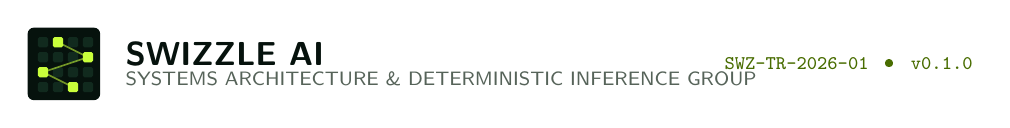
\begin{tikzpicture}[Baseline/.style={baseline=(current bounding box.center)}]
  % Swizzle 4x4 XOR Permutation Matrix Mark (from swizzle_avatar.svg)
  \fill[swzInk, rounded corners=2.2pt] (0,0) rectangle (0.92,0.92);
  \foreach \r in {0,1,2,3} {
    \foreach \c in {0,1,2,3} {
      \pgfmathsetmacro{\x}{0.13 + \c * 0.19}
      \pgfmathsetmacro{\y}{0.67 - \r * 0.19}
      \fill[swzDark, rounded corners=0.6pt] (\x,\y) rectangle (\x+0.13,\y+0.13);
    }
  }
  % Active permutation cells: (0,1), (1,3), (2,0), (3,2)
  \fill[swzLime, rounded corners=0.6pt] (0.32,0.67) rectangle (0.45,0.80);
  \fill[swzLime, rounded corners=0.6pt] (0.70,0.48) rectangle (0.83,0.61);
  \fill[swzLime, rounded corners=0.6pt] (0.13,0.29) rectangle (0.26,0.42);
  \fill[swzLime, rounded corners=0.6pt] (0.51,0.10) rectangle (0.64,0.23);
  % Trace vectors
  \draw[swzLime, line width=0.6pt, opacity=0.55] (0.385,0.735) -- (0.765,0.545) -- (0.195,0.355) -- (0.575,0.165);

  \node[anchor=west, font=\sffamily\bfseries\large, text=swzInk] at (1.12, 0.58) {SWIZZLE AI};
  \node[anchor=west, font=\sffamily\scriptsize, text=swzMuted] at (1.12, 0.27) {SYSTEMS ARCHITECTURE \& DETERMINISTIC INFERENCE GROUP};
  \node[anchor=east, font=\ttfamily\scriptsize, text=swzOlive] at (\textwidth, 0.46) {SWZ-TR-2026-01 \;\textbullet\; v0.1.0};
\end{tikzpicture}

\vspace{4mm}

{\sffamily\bfseries\fontsize{20.5}{24.5}\selectfont\color{swzInk}
Swizzle Runtime: Exact, High-Throughput Local Language and Vision-Language Inference\par}

\vspace{1.5mm}
{\sffamily\fontsize{11}{14}\selectfont\color{swzMuted}
First-Principles Architecture, Coding Decisions, Bit-Identical Speculative Verification, XOR-Swizzled Tensor-Core Kernels, and Verified Hardware Benchmarks\par}

\vspace{2.5mm}
{\normalsize\textbf{Paramveer Singh} \quad {\small\color{swzMuted}Swizzle AI \;\textbullet\; \texttt{https://github.com/Swizzle-AI/swizzle-runtime}}\par}

\vspace{3mm}

% Abstract Box
\noindent
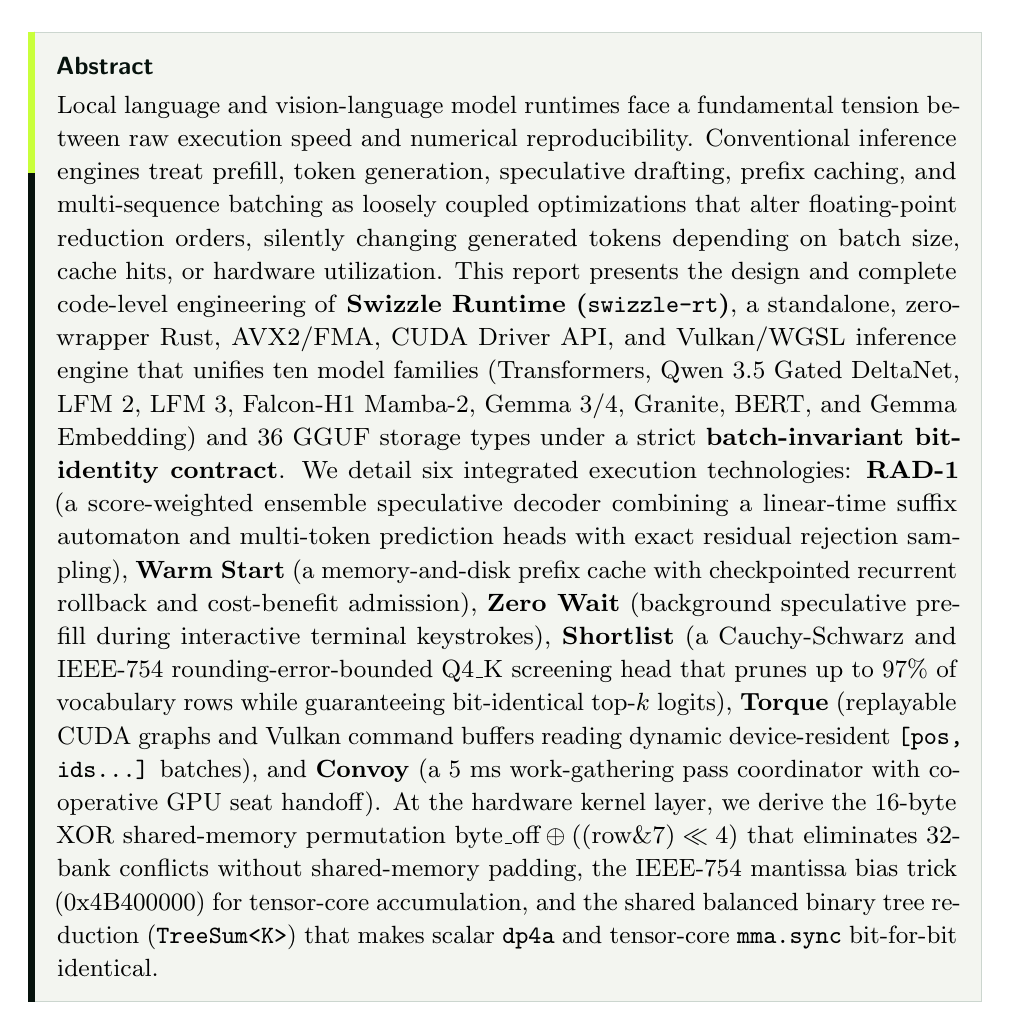
\begin{tikzpicture}
  \node[
    fill=swzBone,
    draw=swzRule,
    line width=0.5pt,
    inner sep=9pt,
    text width=\dimexpr\textwidth-20pt\relax,
    align=justify
  ] (abs) {
    {\sffamily\bfseries\small\color{swzInk}Abstract}\par\vspace{2pt}
    {\small
    Local language and vision-language model runtimes face a fundamental tension between raw execution speed and numerical reproducibility. Conventional inference engines treat prefill, token generation, speculative drafting, prefix caching, and multi-sequence batching as loosely coupled optimizations that alter floating-point reduction orders, silently changing generated tokens depending on batch size, cache hits, or hardware utilization. This report presents the design and complete code-level engineering of \textbf{Swizzle Runtime (\texttt{swizzle-rt})}, a standalone, zero-wrapper Rust, AVX2/FMA, CUDA Driver API, and Vulkan/WGSL inference engine that unifies ten model families (Transformers, Qwen 3.5 Gated DeltaNet, LFM 2, LFM 3, Falcon-H1 Mamba-2, Gemma 3/4, Granite, BERT, and Gemma Embedding) and 36 GGUF storage types under a strict \textbf{batch-invariant bit-identity contract}. We detail six integrated execution technologies: \textbf{RAD-1} (a score-weighted ensemble speculative decoder combining a linear-time suffix automaton and multi-token prediction heads with exact residual rejection sampling), \textbf{Warm Start} (a memory-and-disk prefix cache with checkpointed recurrent rollback and cost-benefit admission), \textbf{Zero Wait} (background speculative prefill during interactive terminal keystrokes), \textbf{Shortlist} (a Cauchy-Schwarz and IEEE-754 rounding-error-bounded $\text{Q4\_K}$ screening head that prunes up to $97\%$ of vocabulary rows while guaranteeing bit-identical top-$k$ logits), \textbf{Torque} (replayable CUDA graphs and Vulkan command buffers reading dynamic device-resident \texttt{[pos, ids...]} batches), and \textbf{Convoy} (a $5\text{ ms}$ work-gathering pass coordinator with cooperative GPU seat handoff). At the hardware kernel layer, we derive the $16\text{-byte}$ XOR shared-memory permutation $\text{byte\_off} \oplus ((\text{row} \& 7) \ll 4)$ that eliminates 32-bank conflicts without shared-memory padding, the IEEE-754 mantissa bias trick ($0\text{x}4\text{B}400000$) for tensor-core accumulation, and the shared balanced binary tree reduction (\texttt{TreeSum<K>}) that makes scalar \texttt{dp4a} and tensor-core \texttt{mma.sync} bit-for-bit identical.}
  };
  \draw[swzInk, line width=2.8pt] (abs.north west) -- (abs.south west);
  \draw[swzLime, line width=2.8pt] (abs.north west) -- ([yshift=-18mm]abs.north west);
\end{tikzpicture}

\vspace{2.5mm}

% 4 Hero Stat Callout Cards
\noindent
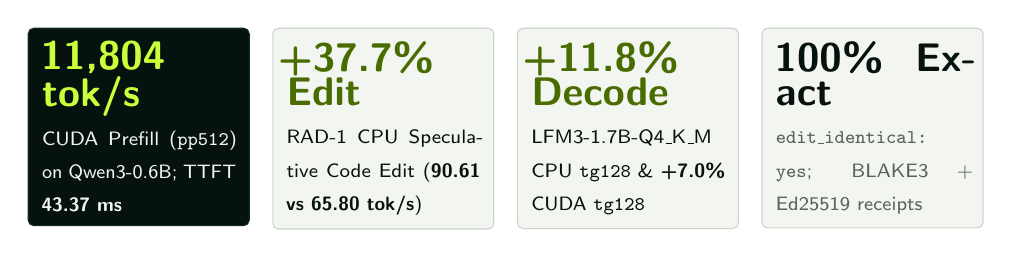
\begin{tikzpicture}
  \pgfmathsetmacro{\w}{(\textwidth - 9mm)/4}
  \node[fill=swzInk, draw=swzDark, rounded corners=2pt, minimum width=\w pt, minimum height=17.5mm, inner sep=5pt, anchor=north west] (c1) at (0,0) {
    \begin{minipage}{\dimexpr\w pt - 10pt\relax}
      {\sffamily\bfseries\fontsize{14}{16}\selectfont\color{swzLime}11,804 tok/s}\\[2pt]
      {\sffamily\scriptsize\color{swzBone}CUDA Prefill (\texttt{pp512}) on Qwen3-0.6B; TTFT \textbf{43.37 ms}}
    \end{minipage}
  };
  \node[fill=swzBone, draw=swzRule, rounded corners=2pt, minimum width=\w pt, minimum height=17.5mm, inner sep=5pt, anchor=north west] (c2) at (\w pt + 3mm, 0) {
    \begin{minipage}{\dimexpr\w pt - 10pt\relax}
      {\sffamily\bfseries\fontsize{14}{16}\selectfont\color{swzOlive}+37.7\% Edit}\\[2pt]
      {\sffamily\scriptsize\color{swzInk}RAD-1 CPU Speculative Code Edit (\textbf{90.61 vs 65.80 tok/s})}
    \end{minipage}
  };
  \node[fill=swzBone, draw=swzRule, rounded corners=2pt, minimum width=\w pt, minimum height=17.5mm, inner sep=5pt, anchor=north west] (c3) at (2*\w pt + 6mm, 0) {
    \begin{minipage}{\dimexpr\w pt - 10pt\relax}
      {\sffamily\bfseries\fontsize{14}{16}\selectfont\color{swzOlive}+11.8\% Decode}\\[2pt]
      {\sffamily\scriptsize\color{swzInk}LFM3-1.7B-Q4\_K\_M CPU \texttt{tg128} \& \textbf{+7.0\%} CUDA \texttt{tg128}}
    \end{minipage}
  };
  \node[fill=swzBone, draw=swzRule, rounded corners=2pt, minimum width=\w pt, minimum height=17.5mm, inner sep=5pt, anchor=north west] (c4) at (3*\w pt + 9mm, 0) {
    \begin{minipage}{\dimexpr\w pt - 10pt\relax}
      {\sffamily\bfseries\fontsize{14}{16}\selectfont\color{swzInk}100\% Exact}\\[2pt]
      {\sffamily\scriptsize\color{swzMuted}\texttt{edit\_identical: yes}; BLAKE3 + Ed25519 receipts}
    \end{minipage}
  };
\end{tikzpicture}

\vspace{3mm}

% Figure 1: End-to-End Turn Timeline Comparison (Baseline vs Swizzle Runtime)
\noindent
\begin{tikzpicture}
  \node[anchor=north west, inner sep=0pt] at (0,0) {
    \begin{minipage}{\textwidth}
      {\sffamily\bfseries\footnotesize\color{swzInk}Figure 1. Anatomy of an Interactive Inference Turn: Conventional Runtime vs.\ Swizzle Runtime (\texttt{swizzle-rt})}\\[3pt]
      \begin{tikzpicture}[x=1mm, y=1mm]
        % Background frame
        \fill[swzBone] (0,0) rectangle (166, 36);
        \draw[swzRule, line width=0.5pt] (0,0) rectangle (166, 36);

        % Row 1: Conventional Runtime
        \node[anchor=west, font=\sffamily\bfseries\scriptsize, text=swzInk] at (3, 29.5) {Conventional Engine};
        \node[anchor=west, font=\sffamily\tiny, text=swzMuted] at (3, 26) {(Cold prefill + 1-tok decode)};

        \fill[swzSage, draw=swzRule] (42, 24.5) rectangle (66, 31.5);
        \node[font=\sffamily\tiny, text=swzMuted] at (54, 28) {User Typing (GPU Idle)};

        \draw[-{Stealth[length=1.8mm]}, swzCoral, thick] (66, 33.5) -- (66, 31.6);
        \node[anchor=south, font=\sffamily\bfseries\tiny, text=swzCoral] at (66, 33.2) {Enter};

        \fill[swzLoss, draw=swzCoral] (66, 24.5) rectangle (98, 31.5);
        \node[font=\sffamily\bfseries\tiny, text=swzCoral] at (82, 28) {Cold Prefill (TTFT)};

        \fill[white, draw=swzCoral] (98, 24.5) rectangle (149, 31.5);
        \node[font=\sffamily\tiny, text=swzInk] at (123.5, 28) {1-Token Decode + Full Vocab GEMV};

        \node[anchor=west, font=\ttfamily\bfseries\scriptsize, text=swzCoral] at (150.5, 28) {1.00x};

        % Divider
        \draw[swzRule, dashed] (3, 18.5) -- (163, 18.5);

        % Row 2: Swizzle Runtime
        \node[anchor=west, font=\sffamily\bfseries\scriptsize, text=swzInk] at (3, 12.5) {Swizzle Runtime};
        \node[anchor=west, font=\sffamily\tiny, text=swzOlive] at (3, 9) {(Warm + Zero Wait + RAD-1)};

        \fill[swzGainMid, draw=swzOlive] (42, 7.5) rectangle (53, 14.5);
        \node[font=\sffamily\bfseries\tiny, text=swzInk] at (47.5, 11) {Warm};

        \fill[swzGainHi, draw=swzOlive] (53, 7.5) rectangle (66, 14.5);
        \node[font=\sffamily\bfseries\tiny, text=swzInk] at (59.5, 11) {Zero Wait};

        \draw[-{Stealth[length=1.8mm]}, swzOlive, thick] (66, 16.5) -- (66, 14.6);
        \node[anchor=south, font=\sffamily\bfseries\tiny, text=swzOlive] at (66, 16.2) {Enter (0 ms)};

        \fill[swzInk, draw=swzDark] (66, 7.5) rectangle (103, 14.5);
        \node[font=\sffamily\bfseries\tiny, text=swzLime] at (84.5, 11) {RAD-1 + Torque + Shortlist};

        \draw[{Stealth[length=1.5mm]}-{Stealth[length=1.5mm]}, swzOlive, thick] (104, 11) -- (149, 11);
        \node[fill=swzBone, inner sep=1pt, font=\sffamily\bfseries\tiny, text=swzOlive] at (126.5, 11) {Wall-Clock Time Saved};

        % Bottom time axis
        \draw[-{Stealth[length=1.5mm]}, swzMuted] (42, 3.2) -- (162, 3.2);
        \node[anchor=east, font=\sffamily\tiny, text=swzMuted] at (41, 3.2) {Timeline};
      \end{tikzpicture}
    \end{minipage}
  };
\end{tikzpicture}

\newpage

% ==================== PAGE 2: KEY RESULTS & TABLE OF CONTENTS ====================
\noindent
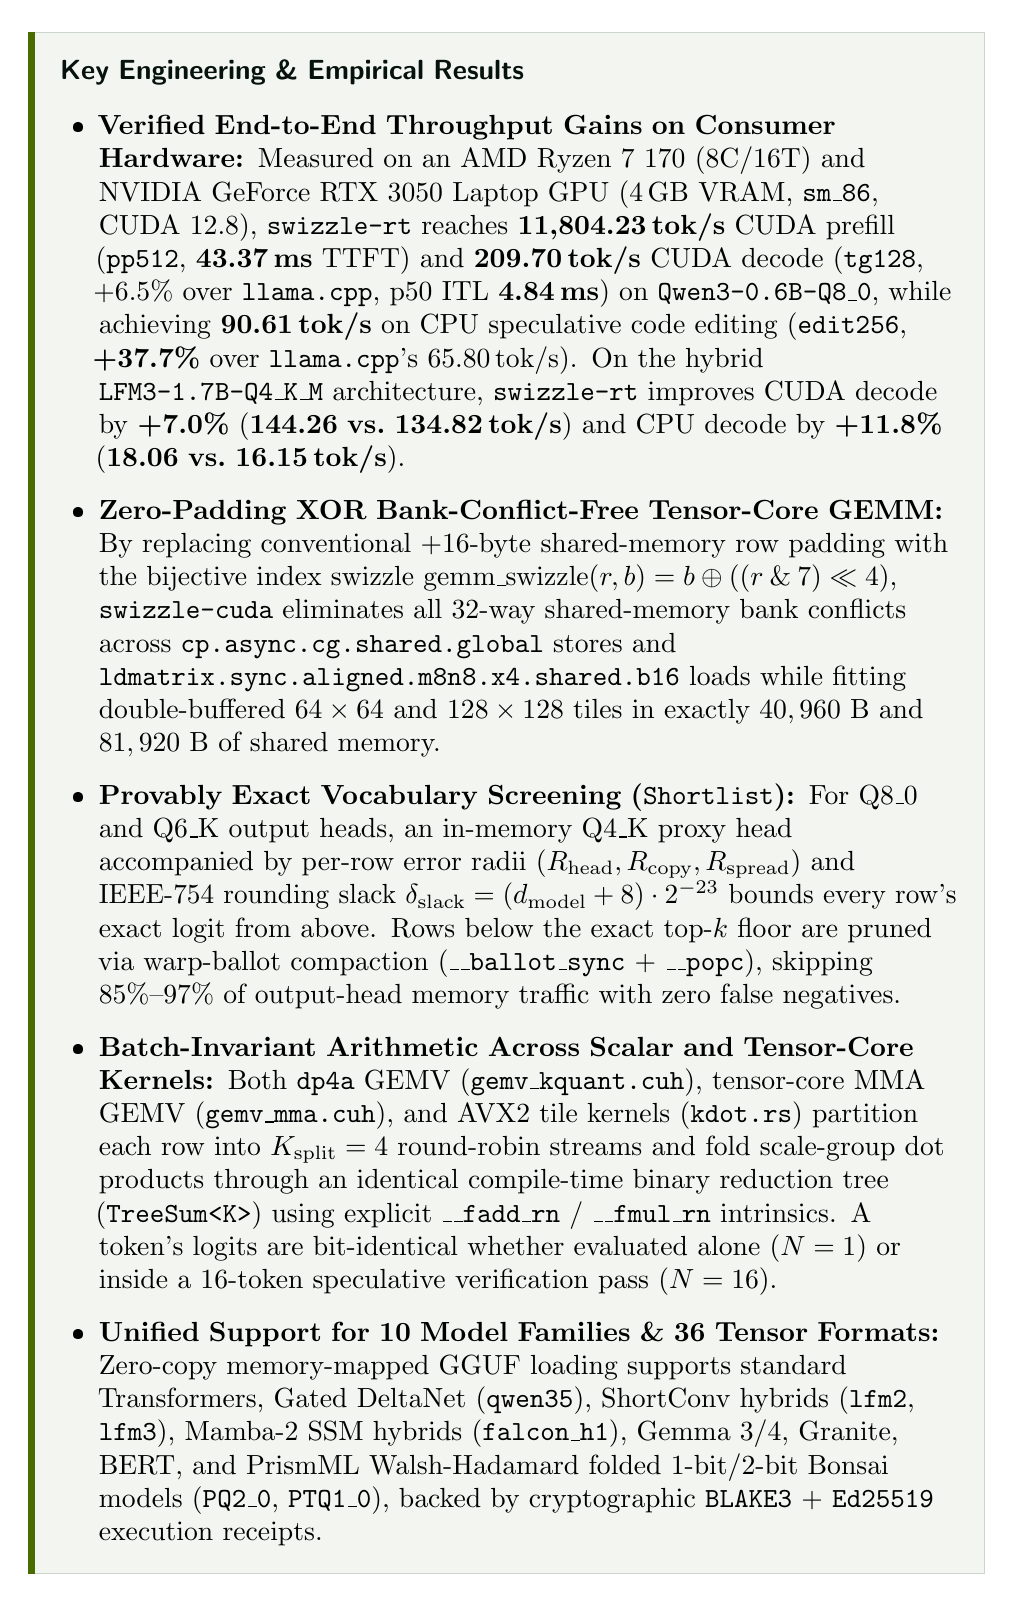
\begin{tikzpicture}
  \node[
    fill=swzBone,
    draw=swzRule,
    line width=0.6pt,
    inner sep=10pt,
    text width=\dimexpr\textwidth-21pt\relax
  ] (kr) {
    {\sffamily\bfseries\normalsize\color{swzInk}Key Engineering \& Empirical Results}\par\vspace{4pt}
    \begin{itemize}[leftmargin=14pt, itemsep=3pt, topsep=2pt]
      \item \textbf{Verified End-to-End Throughput Gains on Consumer Hardware:} Measured on an AMD Ryzen 7 170 (8C/16T) and NVIDIA GeForce RTX 3050 Laptop GPU (4\,GB VRAM, \texttt{sm\_86}, CUDA 12.8), \texttt{swizzle-rt} reaches \textbf{11,804.23\,tok/s} CUDA prefill (\texttt{pp512}, \textbf{43.37\,ms} TTFT) and \textbf{209.70\,tok/s} CUDA decode (\texttt{tg128}, $+6.5\%$ over \texttt{llama.cpp}, p50 ITL \textbf{4.84\,ms}) on \texttt{Qwen3-0.6B-Q8\_0}, while achieving \textbf{90.61\,tok/s} on CPU speculative code editing (\texttt{edit256}, \textbf{+37.7\%} over \texttt{llama.cpp}'s 65.80\,tok/s). On the hybrid \texttt{LFM3-1.7B-Q4\_K\_M} architecture, \texttt{swizzle-rt} improves CUDA decode by \textbf{+7.0\%} (\textbf{144.26 vs.\ 134.82\,tok/s}) and CPU decode by \textbf{+11.8\%} (\textbf{18.06 vs.\ 16.15\,tok/s}).
      \item \textbf{Zero-Padding XOR Bank-Conflict-Free Tensor-Core GEMM:} By replacing conventional $+16\text{-byte}$ shared-memory row padding with the bijective index swizzle $\text{gemm\_swizzle}(r, b) = b \oplus ((r \mathbin{\&} 7) \ll 4)$, \texttt{swizzle-cuda} eliminates all 32-way shared-memory bank conflicts across \texttt{cp.async.cg.shared.global} stores and \texttt{ldmatrix.sync.aligned.m8n8.x4.shared.b16} loads while fitting double-buffered $64\times 64$ and $128\times 128$ tiles in exactly $40,960\text{ B}$ and $81,920\text{ B}$ of shared memory.
      \item \textbf{Provably Exact Vocabulary Screening (\texttt{Shortlist}):} For $\text{Q8\_0}$ and $\text{Q6\_K}$ output heads, an in-memory $\text{Q4\_K}$ proxy head accompanied by per-row error radii $(R_{\text{head}}, R_{\text{copy}}, R_{\text{spread}})$ and IEEE-754 rounding slack $\delta_{\text{slack}} = (d_{\text{model}} + 8)\cdot 2^{-23}$ bounds every row's exact logit from above. Rows below the exact top-$k$ floor are pruned via warp-ballot compaction (\texttt{\_\_ballot\_sync} + \texttt{\_\_popc}), skipping $85\%\text{--}97\%$ of output-head memory traffic with zero false negatives.
      \item \textbf{Batch-Invariant Arithmetic Across Scalar and Tensor-Core Kernels:} Both \texttt{dp4a} GEMV (\texttt{gemv\_kquant.cuh}), tensor-core MMA GEMV (\texttt{gemv\_mma.cuh}), and AVX2 tile kernels (\texttt{kdot.rs}) partition each row into $K_{\text{split}}=4$ round-robin streams and fold scale-group dot products through an identical compile-time binary reduction tree (\texttt{TreeSum<K>}) using explicit \texttt{\_\_fadd\_rn} / \texttt{\_\_fmul\_rn} intrinsics. A token's logits are bit-identical whether evaluated alone ($N=1$) or inside a 16-token speculative verification pass ($N=16$).
      \item \textbf{Unified Support for 10 Model Families \& 36 Tensor Formats:} Zero-copy memory-mapped GGUF loading supports standard Transformers, Gated DeltaNet (\texttt{qwen35}), ShortConv hybrids (\texttt{lfm2}, \texttt{lfm3}), Mamba-2 SSM hybrids (\texttt{falcon\_h1}), Gemma 3/4, Granite, BERT, and PrismML Walsh-Hadamard folded 1-bit/2-bit Bonsai models (\texttt{PQ2\_0}, \texttt{PTQ1\_0}), backed by cryptographic \texttt{BLAKE3} + \texttt{Ed25519} execution receipts.
    \end{itemize}
  };
  \draw[swzOlive, line width=2.8pt] (kr.north west) -- (kr.south west);
\end{tikzpicture}

\vspace{3mm}
{\small
\renewcommand{\contentsname}{\sffamily\bfseries\large\color{swzInk}Contents}
\tableofcontents
}
\newpage

% ==================== SECTION 1: INTRODUCTION ====================
\section{Introduction and First-Principles Design Philosophy}

Local language and vision-language model inference engines operate across two fundamentally distinct hardware regimes during a single user request. During \textbf{prompt prefill}, the runtime processes $N \gg 1$ input tokens simultaneously; each weight matrix $W \in \mathbb{R}^{R \times C}$ is loaded once from DRAM or VRAM and multiplied against an activation matrix $X \in \mathbb{R}^{C \times N}$, making execution compute-bound on SIMD vector units or GPU Tensor Cores. During \textbf{autoregressive token generation (decode)}, the runtime processes $N = 1$ token per step; the entire parameter footprint of the model must be streamed across the memory bus to produce a single output vector $y = Wx$, rendering decode strictly memory-bandwidth-bound.

For a dense model of $B_{\text{weights}}$ bytes running on a memory subsystem with sustained bandwidth $\text{BW}_{\text{mem}}$ and efficiency $\eta \in [0.55, 0.85]$, the theoretical ceiling on single-token decode throughput is governed by the memory-bandwidth roofline:
\begin{equation}
  T_{\text{decode}}^{\max} = \frac{\eta \cdot \text{BW}_{\text{mem}}}{B_{\text{weights}} + B_{\text{KV}}(L_{\text{ctx}})}
  \label{eq:roofline_ceiling}
\end{equation}
where $B_{\text{KV}}(L_{\text{ctx}})$ is the per-step key-value or recurrent state traffic at context length $L_{\text{ctx}}$. In \code{swizzle-cli/src/fit.rs}, Swizzle Runtime codifies this physical law directly into its hardware planner:
\begin{lstlisting}[language=Rust]
const HEADROOM: u64 = 1 << 30;
/// Decode reaches this share of memory bandwidth, low to high; Swizzle
/// measured 0.70-0.77 on an RTX 3060 and ~0.6 on DDR5.
const GPU_EFFICIENCY: (f64, f64) = (0.55, 0.85);
const CPU_EFFICIENCY: (f64, f64) = (0.45, 0.75);
\end{lstlisting}

\begin{figure}[htbp]
  \centering
  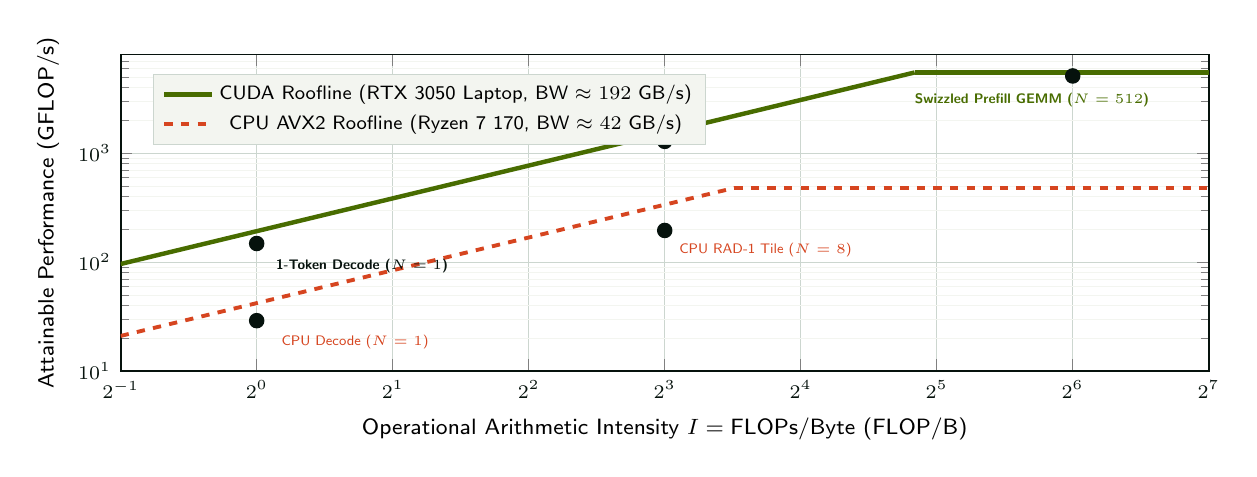
\begin{tikzpicture}
    \begin{axis}[
      width=15.4cm,
      height=5.6cm,
      xmode=log,
      ymode=log,
      log basis x=2,
      log basis y=10,
      xmin=0.5, xmax=128,
      ymin=10, ymax=8000,
      xlabel={\sffamily\footnotesize Operational Arithmetic Intensity $I = \text{FLOPs} / \text{Byte}$ (FLOP/B)},
      ylabel={\sffamily\footnotesize Attainable Performance (GFLOP/s)},
      grid=both,
      major grid style={color=swzRule, line width=0.4pt},
      minor grid style={color=swzBone, line width=0.2pt},
      axis line style={color=swzInk, line width=0.6pt},
      tick label style={font=\sffamily\scriptsize, text=swzInk},
      legend style={at={(0.03,0.94)}, anchor=north west, font=\sffamily\scriptsize, fill=swzBone, draw=swzRule}
    ]
      % GPU Roofline (RTX 3050 Laptop: ~192 GB/s BW, ~5500 GFLOP/s effective INT8/FP16 kernel ceiling)
      \addplot[color=swzOlive, line width=1.6pt, domain=0.5:28.6] {192 * x};
      \addplot[color=swzOlive, line width=1.6pt, domain=28.6:128, forget plot] {5500};
      \addlegendentry{CUDA Roofline (RTX 3050 Laptop, $\text{BW}\approx 192\text{ GB/s}$)}

      % CPU Roofline (Ryzen 7 170 DDR5: ~42 GB/s BW, ~480 GFLOP/s AVX2 ceiling)
      \addplot[color=swzCoral, line width=1.4pt, dashed, domain=0.5:11.4] {42 * x};
      \addplot[color=swzCoral, line width=1.4pt, dashed, domain=11.4:128, forget plot] {480};
      \addlegendentry{CPU AVX2 Roofline (Ryzen 7 170, $\text{BW}\approx 42\text{ GB/s}$)}

      % Operating regimes
      \addplot[only marks, mark=*, mark size=2.6pt, color=swzInk] coordinates {
        (1.0, 148)
        (8.0, 1280)
        (64.0, 5100)
        (1.0, 29)
        (8.0, 195)
      };
      \node[anchor=north west, font=\sffamily\bfseries\tiny, text=swzInk] at (axis cs:1.05,130) {1-Token Decode ($N=1$)};
      \node[anchor=south east, font=\sffamily\bfseries\tiny, text=swzOlive] at (axis cs:7.5,1350) {RAD-1 Verify ($N=8$)};
      \node[anchor=north, font=\sffamily\bfseries\tiny, text=swzOlive] at (axis cs:52,4400) {Swizzled Prefill GEMM ($N=512$)};
      \node[anchor=north west, font=\sffamily\tiny, text=swzCoral] at (axis cs:1.08,26) {CPU Decode ($N=1$)};
      \node[anchor=north west, font=\sffamily\tiny, text=swzCoral] at (axis cs:8.2,185) {CPU RAD-1 Tile ($N=8$)};
    \end{axis}
  \end{tikzpicture}
  \caption{Roofline operational regimes of \texttt{swizzle-rt} on the benchmarked RTX 3050 Laptop GPU and Ryzen 7 170 CPU. Single-token decode ($N=1$) sits at $I \approx 1\text{ FLOP/B}$ on the memory-bandwidth slope; \textbf{RAD-1} speculative verification and \textbf{Convoy} batching shift execution up the slope ($N=4\text{--}16$) by amortizing each weight read across multiple tokens.}
  \label{fig:roofline}
\end{figure}

Because Equation~(\ref{eq:roofline_ceiling}) is bounded by physical memory bandwidth when $N=1$, an inference engine can only surpass the single-token memory wall through four orthogonal mechanisms:
\begin{enumerate}
  \item \textbf{Maximize $\eta$ (Kernel \& Launch Efficiency):} Stream weights with L1-evict-first cache hints (\code{\_\_ldcs}), keep reused quantized activations in L1/shared memory (\code{\_\_ldg}), eliminate shared-memory bank conflicts via XOR address swizzling, cap CPU decode threads to physical cores to prevent L2/L3 cache thrashing, and capture entire decode passes into replayable \textbf{Torque} CUDA graphs or Vulkan command buffers.
  \item \textbf{Reduce $B_{\text{weights}}$ Read per Step (\texttt{Shortlist}):} Screen the vocabulary projection matrix $W_{\text{head}} \in \mathbb{R}^{V \times d}$ using a compact $\text{Q4\_K}$ proxy and rigorous error bounds so that $85\%\text{--}97\%$ of full-precision $\text{Q8\_0}$ or $\text{Q6\_K}$ vocabulary rows are never fetched from memory.
  \item \textbf{Increase Tokens Produced per Weight Pass (\texttt{RAD-1} \& \texttt{Convoy}):} Propose $k$ draft tokens per step via an ensemble of suffix-automaton context lookup and multi-token prediction (MTP) heads, verifying all $1+k$ tokens in a single batched weight read, or gather concurrent client requests within a $5\text{ ms}$ \textbf{Convoy} window.
  \item \textbf{Eliminate Redundant Prefill Passes (\texttt{Warm Start} \& \texttt{Zero Wait}):} Persist exact attention KV and recurrent checkpoints in memory and on disk so repeated system prompts resume immediately, and run the user's draft message through the model \emph{while they are still typing} in the terminal so Time-To-First-Token (TTFT) upon pressing Enter approaches zero.
\end{enumerate}

\subsection{The Batch-Invariance \& Exactness Contract}

In almost all existing LLM runtimes, turning on speculative decoding, continuous batching, or tensor-core GEMV subtly alters the generated text. The root cause is IEEE-754 floating-point non-associativity: $(a + b) + c \neq a + (b + c)$. When a single-token decode step uses a warp-per-row scalar \code{dp4a} reduction, while an 8-token speculative verification step dispatches a tiled Tensor Core \code{mma.sync} kernel that accumulates across different $K$-blocks, rounding discrepancies accumulate across layers and flip greedy \code{argmax} or softmax draws.

\begin{invariant}[Swizzle Batch-Invariance Contract]
Let $f(x_1, \dots, x_t)$ denote the output logit vector at position $t$. In \texttt{swizzle-rt}, every quantized GEMV, MMA GEMV, AVX2 tile kernel, chunked attention kernel, and recurrent mixer is engineered so that the floating-point operations producing token $t$'s output occur in an \textbf{identical parenthesization and rounding order} regardless of batch size $N \in [1, \text{MAX\_BATCH}]$, regardless of whether \texttt{dp4a} or \texttt{mma.sync} is selected, and regardless of whether \texttt{Shortlist}, \texttt{RAD-1}, \texttt{Torque}, or \texttt{Convoy} is active.
\end{invariant}

\begin{table}[htbp]
  \centering
  \caption{The Six Speed Technologies of Swizzle Runtime (\texttt{swizzle-cli/src/tech.rs}) and Their Hardware Scope.}
  \label{tab:six_technologies}
  \small
  \begin{tabularx}{\textwidth}{@{}llccX@{}}
    \toprule
    \sffamily\bfseries Flag (\texttt{--off}) & \sffamily\bfseries Public Name & \sffamily\bfseries CPU & \sffamily\bfseries CUDA / Vulkan & \sffamily\bfseries Core Mechanism \& Exactness Guarantee \\
    \midrule
    \code{rad-1} & \textbf{RAD-1} & Yes & Yes / Yes & Score-weighted ensemble speculative decoding (\code{Lookup} + \code{SessionIndex} SAM + \code{MtpDrafter}) with residual rejection sampling; bit-identical to 1-token decoding. \\
    \code{warm-start} & \textbf{Warm Start} & Yes & Yes / Yes & In-memory (1\,GiB) + disk (2\,GiB \code{.kwarm}) prefix cache with grid-aligned recurrent checkpoints (\code{GRID = 256}) and cost-benefit admission. \\
    \code{zero-wait} & \textbf{Zero Wait} & Yes & Yes / No & Background Condvar thread (\code{ahead.rs}) that prefills the conversation + live keystroke line into the Warm Start cache before Enter is pressed. \\
    \code{shortlist} & \textbf{Shortlist} & Yes & GPU API & $\text{Q4\_K}$ proxy output head with proven per-row L2 error radii $(R_{\text{head}}, R_{\text{copy}}, R_{\text{spread}})$ and IEEE-754 slack; bit-identical top-$k$ / greedy token selection. \\
    \code{torque} & \textbf{Torque} & N/A & Yes / Always & Captures full multi-layer decode passes into a single \code{CUgraphExec} or Vulkan \code{VkCommandBuffer} reading device-resident \code{[pos, ids...]}. \\
    \code{convoy} & \textbf{Convoy} & Yes & Yes / No & Multi-sequence work-gathering coordinator (\code{GATHER = 5\,ms}) with RAII \code{Seat::away} GPU lock release during slow client socket writes. \\
    \bottomrule
  \end{tabularx}
\end{table}

% ==================== SECTION 2: SYSTEM ARCHITECTURE ====================
\section{System Architecture and Crate Workspace}

Swizzle Runtime is organized as a Cargo workspace (\code{edition = "2021"}, \code{rust-version = "1.91"}, \code{lto = "thin"}, \code{codegen-units = 1}) comprising ten focused Rust crates with minimal external dependencies (\code{half = "2"}, \code{rayon = "1"}, \code{memmap2 = "0.9"}). Neither \code{llama.cpp}, \code{ggml}, \code{cudart}, nor the Vulkan SDK is linked at build or runtime; all hardware drivers (\code{nvcuda.dll}/\code{libcuda.so.1} and \code{vulkan-1.dll}/\code{libvulkan.so.1}) are resolved dynamically via function-pointer tables.

\begin{figure}[htbp]
  \centering
  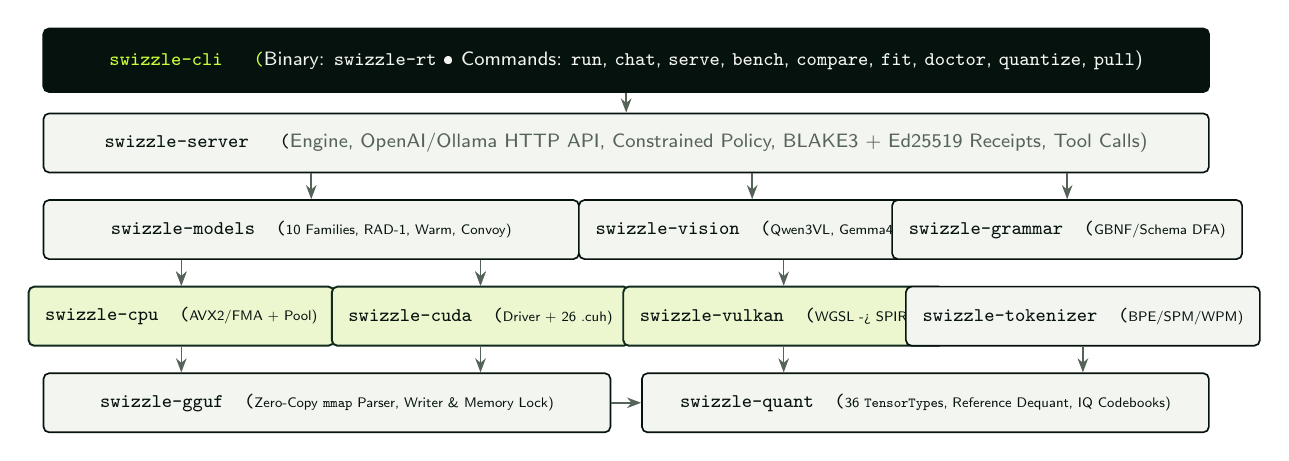
\begin{tikzpicture}[
    crate/.style={draw=swzInk, line width=0.6pt, fill=swzBone, rounded corners=2pt, minimum height=7.5mm, inner xsep=6pt, font=\ttfamily\bfseries\scriptsize, text=swzInk},
    hwcrate/.style={draw=swzDark, line width=0.7pt, fill=swzGainMid, rounded corners=2pt, minimum height=7.5mm, inner xsep=6pt, font=\ttfamily\bfseries\scriptsize, text=swzInk},
    topcrate/.style={draw=swzInk, line width=0.8pt, fill=swzInk, rounded corners=2pt, minimum height=8mm, inner xsep=8pt, font=\ttfamily\bfseries\scriptsize, text=swzLime},
    arr/.style={-{Stealth[length=1.8mm]}, draw=swzMuted, line width=0.55pt}
  ]
    % Layer 5: CLI
    \node[topcrate, minimum width=148mm] (cli) at (0, 3.8) {swizzle-cli \quad (\normalfont\sffamily\scriptsize\color{swzBone}Binary: \texttt{swizzle-rt} \textbullet\ Commands: \texttt{run}, \texttt{chat}, \texttt{serve}, \texttt{bench}, \texttt{compare}, \texttt{fit}, \texttt{doctor}, \texttt{quantize}, \texttt{pull})};

    % Layer 4: Server
    \node[crate, minimum width=148mm] (srv) at (0, 2.75) {swizzle-server \quad (\normalfont\sffamily\scriptsize\color{swzMuted}Engine, OpenAI/Ollama HTTP API, Constrained Policy, BLAKE3 + Ed25519 Receipts, Tool Calls)};

    % Layer 3: Models & Vision & Grammar
    \node[crate, minimum width=68mm] (mod) at (-4.0, 1.65) {swizzle-models \ (\normalfont\sffamily\tiny 10 Families, RAD-1, Warm, Convoy)};
    \node[crate, minimum width=38mm] (vis) at (1.6, 1.65) {swizzle-vision \ (\normalfont\sffamily\tiny Qwen3VL, Gemma4V)};
    \node[crate, minimum width=36mm] (grm) at (5.6, 1.65) {swizzle-grammar \ (\normalfont\sffamily\tiny GBNF/Schema DFA)};

    % Layer 2: Backends & Tokenizer
    \node[hwcrate, minimum width=35mm] (cpu) at (-5.65, 0.55) {swizzle-cpu \ (\normalfont\sffamily\tiny AVX2/FMA + Pool)};
    \node[hwcrate, minimum width=37mm] (cuda) at (-1.85, 0.55) {swizzle-cuda \ (\normalfont\sffamily\tiny Driver + 26 .cuh)};
    \node[hwcrate, minimum width=36mm] (vk) at (2.0, 0.55) {swizzle-vulkan \ (\normalfont\sffamily\tiny WGSL -> SPIR-V)};
    \node[crate, minimum width=32mm] (tok) at (5.8, 0.55) {swizzle-tokenizer \ (\normalfont\sffamily\tiny BPE/SPM/WPM)};

    % Layer 1: Foundation
    \node[crate, minimum width=72mm] (gguf) at (-3.8, -0.55) {swizzle-gguf \ (\normalfont\sffamily\tiny Zero-Copy \texttt{mmap} Parser, Writer \& Memory Lock)};
    \node[crate, minimum width=72mm] (qnt) at (3.8, -0.55) {swizzle-quant \ (\normalfont\sffamily\tiny 36 \texttt{TensorType}s, Reference Dequant, IQ Codebooks)};

    % Arrows
    \draw[arr] (cli) -- (srv);
    \draw[arr] (srv.south -| mod.north) -- (mod.north);
    \draw[arr] (srv.south -| vis.north) -- (vis.north);
    \draw[arr] (srv.south -| grm.north) -- (grm.north);
    \draw[arr] (mod.south -| cpu.north) -- (cpu.north);
    \draw[arr] (mod.south -| cuda.north) -- (cuda.north);
    \draw[arr] (mod.south -| vk.north) -- (vk.north);
    \draw[arr] (vis.south -| cpu.north) -- (cpu.north);
    \draw[arr] (vis.south -| cuda.north) -- (cuda.north);
    \draw[arr] (cpu.south) -- (cpu.south |- qnt.north);
    \draw[arr] (cuda.south) -- (cuda.south |- qnt.north);
    \draw[arr] (vk.south) -- (vk.south |- qnt.north);
    \draw[arr] (tok.south) -- (tok.south |- gguf.north);
    \draw[arr] (gguf.east) -- (qnt.west);
  \end{tikzpicture}
  \caption{Dependency DAG of the ten crates in the \texttt{swizzle-runtime} workspace. Every hardware kernel in \texttt{swizzle-cpu}, \texttt{swizzle-cuda}, and \texttt{swizzle-vulkan} is verified against the scalar reference dequantizer in \texttt{swizzle-quant}.}
  \label{fig:crate_dag}
\end{figure}

\begin{table}[htbp]
  \centering
  \caption{Crate Responsibilities and Key Modules Across the \texttt{swizzle-runtime} Workspace.}
  \label{tab:crate_breakdown}
  \small
  \begin{tabularx}{\textwidth}{@{}llX@{}}
    \toprule
    \sffamily\bfseries Crate & \sffamily\bfseries Core Modules & \sffamily\bfseries Engineering Scope \& Architectural Invariants \\
    \midrule
    \code{swizzle-quant} & \code{types}, \code{dequant}, \code{encode}, \code{grids}, \code{iq}, \code{matrix} & Defines all 36 GGUF \code{TensorType} discriminants, scalar reference \code{dequantize\_row}, quantization encoders, and IQ codebook tables (\code{IQ1S}, \code{IQ2XXS}, \code{IQ2XS}, \code{IQ2S}, \code{IQ3XXS}, \code{IQ3S}, \code{IQ4NL}). \\
    \code{swizzle-gguf} & \code{reader}, \code{writer}, \code{value}, \code{file\_type}, \code{lock} & Validates GGUF v2/v3 headers against buffer bounds before zero-copy \code{memmap2} slicing; enforces 32-byte alignment (\code{DEFAULT\_ALIGNMENT = 32}) and optional OS page locking. \\
    \code{swizzle-tokenizer} & \code{bpe}, \code{spm}, \code{wpm}, \code{pretokenize}, \code{stream} & Exact llama.cpp-compatible Byte-Level BPE (\code{gpt2} with 11 pre-tokenizers including \code{qwen35}, \code{lfm2}, \code{falcon-h1}), SentencePiece (\code{llama}, \code{gemma4}), and WordPiece (\code{bert}). \\
    \code{swizzle-grammar} & \code{gbnf}, \code{schema}, \code{program}, \code{dfa}, \code{matcher}, \code{vocab} & Compiles GBNF grammars and JSON Schemas into a lazily evaluated byte-stack DFA with stack-cut caching (\code{OPEN}, \code{CONTEXT}) over a vocabulary byte trie. \\
    \code{swizzle-cpu} & \code{matmul}, \code{kdot}, \code{fdot}, \code{pool}, \code{q8}, \code{q8k}, \code{ops} & Custom spin-futex physical-core thread pool (\code{pool.rs}), AVX2/FMA 1-token and $N$-token tile kernels, L2-resident $192\text{ KiB}$ unpacked weight tiles, and thread-local activation workspaces. \\
    \code{swizzle-cuda} & \code{driver}, \code{gemv}, \code{gemm}, \code{shortlist}, \code{moe}, \code{graph}, \code{batch} & Runtime-loaded \code{nvcuda} wrapper + fatbin (\code{sm\_75}--\code{sm\_120}) housing 26 \code{.cuh} headers: planar weight layout, \code{dp4a}/\code{mma} GEMV, XOR-swizzled GEMM, FlashAttention, and Shortlist. \\
    \code{swizzle-vulkan} & \code{instance}, \code{device}, \code{pipeline}, \code{commands}, \code{gemv}, \code{delta\_net} & Runtime-loaded Vulkan 1.3 backend; compiles WGSL shaders to SPIR-V via \code{naga} at build time; uses subgroup size 32, packed \code{int8} dot products, and push descriptors. \\
    \code{swizzle-vision} & \code{qwen3vl}, \code{gemma4v}, \code{preprocess}, \code{flash}, \code{device} & Multimodal \code{mmproj} loader and image preprocessor; runs ViT towers with AVX2 FlashAttention or CUDA vision kernels and injects 2D/3D rotary grid positions. \\
    \code{swizzle-models} & \code{arch}, \code{blocks}, \code{speculative}, \code{warm}, \code{head}, \code{convoy}, \code{cuda}, \code{vulkan} & Assembles 10 model families from composable blocks; implements \code{Shortlist}, \code{Warm}, \code{Convoy}, \code{LoRA} load-time merging, Hadamard \code{Folds}, and split CPU/GPU execution. \\
    \code{swizzle-server} & \code{engine}, \code{http}, \code{api}, \code{ollama}, \code{constrained}, \code{receipt} & Streaming chat/completion engine, OpenAI (\code{/v1/chat/completions}) and Ollama (\code{/api/chat}) endpoints, grammar-constrained policy, and signed \code{Receipt} generation. \\
    \bottomrule
  \end{tabularx}
\end{table}

% ==================== SECTION 3: ZERO-COPY GGUF & PLANAR LAYOUT ====================
\section{Zero-Copy GGUF Memory Mapping and Planar Device Layouts}

Model loading in \code{swizzle-gguf} is built around a strict zero-copy invariant: tensor weights on disk are never deserialized into heap-allocated \code{Vec<f32>} buffers. Instead, \code{Gguf::parse} validates every header string, metadata array, and tensor descriptor against the exact byte length of the memory-mapped file \emph{during parsing}.

\subsection{Bounds-Verified Zero-Copy Parsing (\texttt{swizzle-gguf/src/lib.rs})}

Every GGUF file opens with the 4-byte magic constant \code{b"GGUF"} and a version tag (versions 2 and 3 supported), followed by tensor count, metadata key-value count, and an optional \code{general.alignment} metadata key defaulting to \code{DEFAULT\_ALIGNMENT = 32}. For each tensor descriptor, \code{Gguf::parse} computes the exact element count $\prod_{i=0}^{d-1} \text{dims}[i]$, verifies that the innermost dimension $\text{dims}[0]$ is a multiple of the quantization format's block length $\text{ty.block\_len()}$, computes the byte size
\begin{equation}
  \text{size} = \frac{\prod_{i} \text{dims}[i]}{\text{ty.block\_len()}} \times \text{ty.block\_bytes()}
\end{equation}
and checks via checked integer arithmetic that $\text{data\_offset} + \text{offset} + \text{size} \le \text{buf.len()}$ before returning the \code{Gguf} struct. Consequently, \code{GgufFile::tensor\_data} can hand out \code{\&'a [u8]} slices straight from the OS page cache with zero bounds-check panics or heap copies during inference.

\subsection{Planar Device Layout Transformation (\texttt{swizzle-cuda/src/layout.rs})}

While GGUF stores quantized blocks as an \emph{Array of Structures (AoS)} on disk so that each block's scale and quants are adjacent for CPU cache-line streaming, many GGUF block sizes are not multiples of 16 bytes. For example:
\begin{itemize}
  \item $\text{Q8\_0}$ has a 34-byte block: a 2-byte \code{f16} scale $d$ at offset $0$, followed by 32 \code{int8} quants at offset $2..34$.
  \item $\text{Q6\_K}$ has a 210-byte block: 128 bytes of low 4-bit quants (\code{ql} at $0..128$), 64 bytes of high 2-bit quants (\code{qh} at $128..192$), 16 bytes of \code{int8} scales ($192..208$), and a 2-byte \code{f16} super-block scale $d$ ($208..210$).
  \item $\text{Q4\_0}$ has an 18-byte block ($2\text{ B}$ scale + $16\text{ B}$ nibbles); $\text{PQ2\_0}$ has a 34-byte block ($2\text{ B}$ scale + $32\text{ B}$ 2-bit codes).
\end{itemize}

On a CUDA GPU, reading 16 bytes of quants per lane via vectorized 128-bit \code{int4} loads (\code{\_\_ldcs(const int4*)}) requires every quant run to be 16-byte aligned in device memory. In an AoS layout of 34-byte $\text{Q8\_0}$ blocks, block 0's quants start at byte 2 (unaligned!), block 1's at byte 36, and so on, causing hardware misaligned-address exceptions or serial byte loads.

\begin{decisionbox}{Coding Decision: Planar Structure-of-Arrays (SoA) Device Upload (\texttt{layout.rs})}
When \code{DeviceMatrix::upload} transfers a matrix whose block size is not 16-byte aligned onto the GPU, \code{device\_layout(m)} de-interleaves the blocks into contiguous \textbf{planes}, placing all quant payloads first and all scale/metadata fields afterward:
\begin{equation}
  \text{Plane}_k = \bigcup_{b=0}^{B_{\text{total}}-1} \text{Block}_b[\text{start}_k \dots \text{start}_k + \text{len}_k]
\end{equation}
For $\text{Q8\_0}$ (\code{Q8\_0\_FIELDS = \&[(2, 32), (0, 2)]}), Plane 0 holds $32 \times B_{\text{total}}$ bytes of \code{int8} quants (every 16-byte half-block is naturally 16-byte aligned), and Plane 1 holds $2 \times B_{\text{total}}$ bytes of \code{f16} scales starting at byte offset $32 B_{\text{total}}$. For codebook formats (\code{IQ1\_S}, \code{IQ1\_M}, \code{IQ2\_S}, \code{IQ3\_S}), \code{device\_layout} pads the end of the last plane to the next multiple of 16 bytes and appends the constant lookup grid directly into the same device buffer.
\end{decisionbox}

\begin{figure}[htbp]
  \centering
  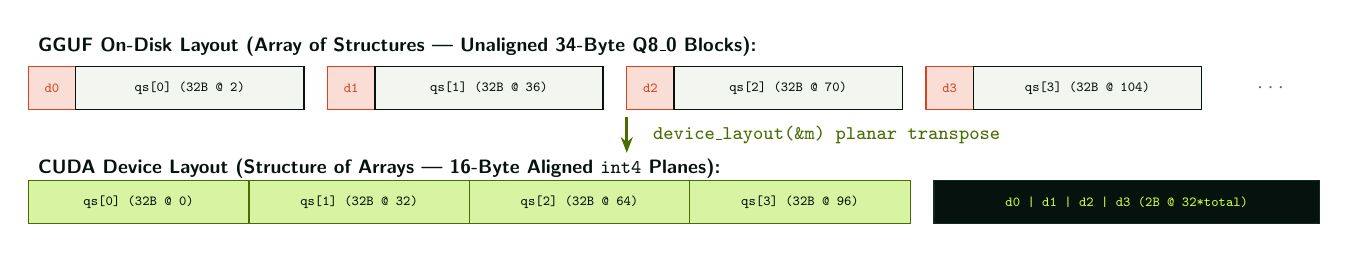
\begin{tikzpicture}[x=1mm, y=1mm]
    % AoS On-Disk Layout
    \node[anchor=west, font=\sffamily\bfseries\scriptsize, text=swzInk] at (0, 22) {GGUF On-Disk Layout (Array of Structures --- Unaligned 34-Byte $\text{Q8\_0}$ Blocks):};
    \foreach \b/\x in {0/0, 1/38, 2/76, 3/114} {
      \fill[swzLoss, draw=swzCoral, line width=0.5pt] (\x, 14) rectangle (\x+6, 19.5);
      \node[font=\ttfamily\tiny, text=swzCoral] at (\x+3, 16.75) {d\b};
      \fill[swzBone, draw=swzInk, line width=0.5pt] (\x+6, 14) rectangle (\x+35, 19.5);
      \node[font=\ttfamily\tiny, text=swzInk] at (\x+20.5, 16.75) {qs[\b] (32B @ \pgfmathparse{int(\b*34+2)}\pgfmathresult)};
    }
    \node[font=\sffamily\scriptsize, text=swzMuted] at (158, 16.75) {$\cdots$};

    % Arrow
    \draw[-{Stealth[length=2mm]}, swzOlive, line width=1pt] (76, 13) -- (76, 8.5) node[midway, right=2mm, font=\ttfamily\scriptsize, text=swzOlive] {device\_layout(\&m) planar transpose};

    % SoA Device Layout
    \node[anchor=west, font=\sffamily\bfseries\scriptsize, text=swzInk] at (0, 6.5) {CUDA Device Layout (Structure of Arrays --- 16-Byte Aligned \texttt{int4} Planes):};
    \foreach \b/\x in {0/0, 1/28, 2/56, 3/84} {
      \fill[swzGainHi, draw=swzOlive, line width=0.5pt] (\x, -0.5) rectangle (\x+28, 5);
      \node[font=\ttfamily\tiny, text=swzInk] at (\x+14, 2.25) {qs[\b] (32B @ \pgfmathparse{int(\b*32)}\pgfmathresult)};
    }
    \fill[swzInk, draw=swzDark, line width=0.5pt] (115, -0.5) rectangle (164, 5);
    \node[font=\ttfamily\tiny, text=swzLime] at (139.5, 2.25) {d0 | d1 | d2 | d3 (2B @ 32*total)};
  \end{tikzpicture}
  \caption{Transformation from GGUF on-disk AoS blocks to 16-byte aligned planar SoA device memory in \texttt{swizzle-cuda/src/layout.rs}. Every 16-byte half-block in \texttt{qs} is read via a single \texttt{\_\_ldcs(const int4*)} instruction.}
  \label{fig:planar_layout}
\end{figure}

% ==================== SECTION 4: QUANTIZATION TAXONOMY ====================
\section{Quantization Taxonomy: 36 Tensor Formats and Hadamard Folding}

\code{swizzle-quant} implements exact scalar reference dequantization (\code{dequant.rs}) and quantization (\code{encode.rs}) for 36 tensor formats, spanning IEEE/bfloat floats, legacy 32-element block quants, 256-element super-block K-quants, non-linear vector-quantized Importance Quants (IQ), ternary quants, microscaling \code{MXFP4}, and PrismML 1-bit/2-bit formats.

\begin{table}[htbp]
  \centering
  \caption{Complete Taxonomy of the 36 Tensor Storage Types Supported by \texttt{swizzle-quant/src/types.rs}.}
  \label{tab:tensor_types}
  \footnotesize
  \begin{tabularx}{\textwidth}{@{}llrrlX@{}}
    \toprule
    \sffamily\bfseries Family & \sffamily\bfseries \texttt{TensorType} & \sffamily\bfseries ID & \sffamily\bfseries \texttt{block\_len} & \sffamily\bfseries \texttt{block\_bytes} & \sffamily\bfseries Reconstruction Formula \& Bit Packing \\
    \midrule
    \multirow{2}{*}{Dense / Int} & \code{F32}, \code{F64}, \code{I8..I64} & 0,24..28 & 1 & 1--8 B & Unquantized IEEE-754 float or signed integer scalar. \\
    & \code{F16}, \code{BF16} & 1, 30 & 1 & 2 B & IEEE-754 binary16 or brain float16, widened to \code{f32} on load. \\
    \midrule
    \multirow{4}{*}{Legacy (32)} & \code{Q4\_0}, \code{Q4\_1} & 2, 3 & 32 & 18 B, 20 B & $w_i = d(q_i - 8)$ (\code{Q4\_0}) or $d\cdot q_i + m$ (\code{Q4\_1}); lo/hi nibbles in $16\text{ B}$. \\
    & \code{Q5\_0}, \code{Q5\_1} & 6, 7 & 32 & 22 B, 24 B & 4-bit nibbles + 32-bit high-bit mask \code{qh}; $w_i = d(q_i - 16)$ or $d q_i + m$. \\
    & \code{Q8\_0}, \code{Q8\_1} & 8, 9 & 32 & 34 B, 36 B & $w_i = d \cdot q_i$ with $q_i \in [-127, 127]$ (\code{Q8\_1} adds pre-summed $s$). \\
    & \code{IQ4NL}, \code{MXFP4} & 20, 39 & 32 & 18 B, 17 B & Non-linear 16-entry lut \code{IQ4NL\_VALUES} or E8M0 shared exponent + FP4. \\
    \midrule
    \multirow{6}{*}{K-Quants (256)} & \code{Q2\_K} & 10 & 256 & 84 B & 16 groups of 16: 4-bit scale/min bytes, 2-bit quants, \code{f16} $(d, d_{\min})$. \\
    & \code{Q3\_K} & 11 & 256 & 110 B & 16 signed 6-bit scales packed in $12\text{ B}$, 2-bit \code{qs} + 1-bit \code{hm}, $q_i - 4$. \\
    & \code{Q4\_K} & 12 & 256 & 144 B & 8 sub-blocks of 32: 6-bit $(sc_s, m_s)$ in $12\text{ B}$, $w = d\cdot sc_s \cdot q - d_{\min} m_s$. \\
    & \code{Q5\_K} & 13 & 256 & 176 B & Same $12\text{ B}$ 6-bit scale/min header as \code{Q4\_K} + $32\text{ B}$ fifth-bit \code{qh}. \\
    & \code{Q6\_K} & 14 & 256 & 210 B & 16 runs of 16: $128\text{ B}$ \code{ql} + $64\text{ B}$ \code{qh} + $16\text{ B}$ \code{int8} scales + \code{f16} $d$; $(q - 32)$. \\
    & \code{Q8\_K} & 15 & 256 & 292 B & \code{f32} scale $d$, $256\text{ B}$ \code{int8} quants, $16 \times \text{i16}$ sub-block sums. \\
    \midrule
    \multirow{5}{*}{IQ Codebook} & \code{IQ2\_XXS}, \code{IQ2\_XS} & 16, 17 & 256 & 66 B, 74 B & 2.06 / 2.31 bpw: 8-weight codebook grid + 7-bit odd-parity sign byte. \\
    & \code{IQ2\_S}, \code{IQ3\_XXS} & 22, 18 & 256 & 82 B, 98 B & 2.56 / 3.06 bpw: 512-entry \code{IQ2S\_GRID} or 256-entry \code{IQ3XXS\_GRID}. \\
    & \code{IQ3\_S}, \code{IQ4\_XS} & 21, 23 & 256 & 110 B, 136 B & 3.44 / 4.25 bpw: 512-entry \code{IQ3S\_GRID} or 6-bit scaled \code{IQ4NL\_VALUES}. \\
    & \code{IQ1\_S}, \code{IQ1\_M} & 19, 29 & 256 & 50 B, 56 B & 1.56 / 1.75 bpw: ternary $\{-1,0,+1\}^8$ \code{IQ1S\_GRID} with per-group shift. \\
    \midrule
    \multirow{3}{*}{Ternary / 1-2b} & \code{TQ1\_0}, \code{TQ2\_0} & 34, 35 & 256 & 54 B, 66 B & Base-3 ($3^5=243$ per byte) or 2-bit ternary $\{-1, 0, +1\}$ with \code{f16} $d$. \\
    & \code{Q1\_0}, \code{Q2\_0} & 41, 42 & 128, 64 & 18 B, 18 B & Binary $\pm d$ (128 values) or 2-bit $(q - 1.5)d$ (64 values). \\
    & \code{PQ2\_0}, \code{PTQ1\_0} & 142, 143 & 128, 512 & 34 B, 106 B & PrismML Bonsai 2-bit $(q - 1)d$ and 128-scaled base-3 ternary. \\
    \bottomrule
  \end{tabularx}
\end{table}

\subsection{Sub-Block Scale Unpacking in K-Quants (\texttt{kquant.cuh})}

In $\text{Q4\_K}$ (144 bytes per 256 elements) and $\text{Q5\_K}$ (176 bytes per 256 elements), each super-block contains 8 sub-blocks of 32 elements. Each sub-block $s \in \{0, \dots, 7\}$ has a 6-bit unsigned scale $sc_s \in [0, 63]$ and a 6-bit unsigned offset $m_s \in [0, 63]$, packed into 12 bytes immediately following the two \code{f16} super-block scales $(d, d_{\min})$. For $s < 4$, the low 6 bits of byte $s$ hold $sc_s$ and the low 6 bits of byte $s+4$ hold $m_s$. For $s \ge 4$, the low 4 bits of $sc_s$ and $m_s$ are packed into the low and high nibbles of byte $s+4$, while their top 2 bits are stored in the top 2 bits of bytes $s-4$ and $s$. In \code{kquant.cuh}, Swizzle decodes any sub-block $s$ from the three 32-bit little-endian header words $(q_0, q_1, q_2)$ in branch-minimal bit arithmetic:
\begin{lstlisting}[language=C++]
__device__ __forceinline__ int2 k4_scale_min(unsigned s, unsigned q0, unsigned q1, unsigned q2) {
    if (s < 4) return make_int2((q0 >> (8 * s)) & 63, (q1 >> (8 * s)) & 63);
    const unsigned t = 8 * (s - 4);
    return make_int2(((q2 >> t) & 0x0F) | ((q0 >> t >> 2) & 0x30),
                     ((q2 >> t >> 4) & 0x0F) | ((q1 >> t >> 2) & 0x30));
}
\end{lstlisting}

\subsection{PrismML Sylvester-Walsh-Hadamard Folding (\texttt{folds.rs} \& \texttt{prism.cuh})}

Ultra-low-bit quantization formats such as 1-bit (\code{Q1\_0}, \code{PTQ1\_0}) and 2-bit (\code{PQ2\_0}) suffer severe quantization error when weight rows or activations contain heavy-tailed outliers. To disperse outliers uniformly across channels before quantization, PrismML Bonsai models store weights in a rotated basis defined by a block-diagonal Sylvester-Walsh-Hadamard transform with diagonal sign flips $S = \text{diag}(\pm 1)$.

Because the normalized Walsh-Hadamard matrix $H_B \in \mathbb{R}^{B \times B}$ (where $B = 2^k$) is symmetric and orthogonal ($H_B^T H_B = I_B$), inserting $(H_B S)^T (H_B S) = I$ between a weight row $w^T$ and activation vector $x$ preserves their inner product identically:
\begin{equation}
  w^T x = w^T S^T H_B^T H_B S x = (H_B S w)^T (H_B S x) = \tilde{w}^T \tilde{x}
\end{equation}
In \code{swizzle-models/src/folds.rs}, \code{Folds::read} parses the GGUF metadata keys \code{prism.hadamard.*} (\code{version = 1}, \code{transform = "normalized-sylvester-walsh-hadamard"}, \code{block\_size}, \code{sign\_values}, \code{sign\_widths}, \code{weight\_names}, \code{inverse\_weight\_names}). To guarantee that no folded weight tensor is ever accidentally multiplied by an unfolded activation vector, \code{Folds} maintains a \code{claimed: RefCell<HashSet<String>>} registry; after model construction completes, \code{Folds::finish} verifies that every declared tensor in \code{weight\_names} and \code{inverse\_weight\_names} was claimed by a layer block that applies \code{Folding}, returning a hard \code{LoadError} otherwise. On CUDA (\code{prism.cuh}), \code{fold\_rows} multiplies the input by \code{signs[e]}, runs an in-place shared-memory butterfly \code{walsh\_hadamard(v, block)}, scales by \code{\_\_frcp\_rn(\_\_fsqrt\_rn(block))}, and immediately quantizes the rotated activations into $\text{Q8}$ GEMV input blocks in a single fused kernel launch.

% ==================== SECTION 5: CPU ENGINE ====================
\section{CPU Execution Engine: Spin-Futex Pool and AVX2 Tile Kernels}

Standard general-purpose work-stealing thread pools (such as default Rayon configurations) introduce two significant performance hazards during autoregressive LLM decoding:
\begin{enumerate}
  \item \textbf{SMT / Hyper-Threading Cache Thrashing:} During $N=1$ decode, every thread streams distinct rows of the same weight matrix through the per-core L1/L2 caches and saturates the shared DDR5 memory controller. Running two logical SMT threads on the same physical core halves effective L1/L2 capacity per thread and adds pipeline contention without adding memory channels.
  \item \textbf{OS Futex Wakeup Jitter:} A 28-layer model executes roughly $200\text{--}300$ parallel dispatches per generated token (one every $15\text{--}40\,\mu\text{s}$). Putting worker threads to sleep in the OS kernel between dispatches incurs $5\text{--}25\,\mu\text{s}$ of \code{futex}/\code{WaitOnAddress} context-switch latency per barrier.
\end{enumerate}

\subsection{Single-Word Atomic Dispatch and Physical-Core Decode (\texttt{swizzle-cpu/src/pool.rs})}

To eliminate both hazards, \code{swizzle-cpu} implements a custom zero-allocation barrier thread pool in \code{pool.rs}. At startup, \code{physical\_cores()} inspects OS processor topology (parsing \code{/sys/devices/system/cpu/cpu*/topology/core\_cpus\_list} on Linux or calling \code{GetLogicalProcessorInformationEx(RelationProcessorCore)} on Windows) to determine the exact count of physical cores $P_{\text{phys}}$ alongside logical CPUs $P_{\text{logical}}$.

\begin{decisionbox}{Coding Decision: 64-Bit Packed Epoch/Task State \& 2\,ms Hybrid Spin-Park (\texttt{pool.rs})}
All worker coordination is packed into a single 64-bit atomic integer \code{State(AtomicU64)} so that publishing a new parallel job and claiming the first task occur in one lock-free memory operation:
\begin{equation}
  \text{State::pack}(\text{epoch}, \text{tasks}, \text{next}) = (\text{epoch} \ll 32) \;\mathbin{|}\; (\text{tasks} \ll 16) \;\mathbin{|}\; \text{next}
\end{equation}
where bits $63..32$ hold the 32-bit job \code{epoch}, bits $31..16$ hold the total \code{tasks} count ($\le 65,535$), and bits $15..0$ hold the index of the \code{next} unclaimed task. Workers claim tasks via \code{state.0.fetch\_add(1, Ordering::Acquire)}, incrementing the low 16 bits without touching the epoch or task count. Between dispatches, workers spin in userspace for \code{SPIN = Duration::from\_millis(2)} (checking \code{std::hint::spin\_loop()} and calling \code{Instant::now()} only once every \code{YIELD\_EVERY = 256} iterations) before parking on the condvar.
\end{decisionbox}

\begin{lstlisting}[language=Rust]
/// Spin for 2 ms before parking: covers inter-layer gaps during token generation
/// without burning CPU when the server is idle.
const SPIN: Duration = Duration::from_millis(2);
const YIELD_EVERY: u32 = 256;

/// Like [`for_each`], but caps concurrency to physical core count.
/// Memory-bandwidth-bound 1-token GEMV runs faster without SMT cache contention.
pub fn for_each_decode(tasks: usize, body: impl Fn(usize) + Sync) {
    if tasks <= 1 {
        if tasks == 1 { body(0); }
        return;
    }
    let p = pool();
    run_job(p, tasks.min(p.physical), &body);
}
\end{lstlisting}

\subsection{Thread-Local Activation Workspaces and L2-Resident Tile Unpacking (\texttt{matmul.rs})}

During single-token GEMV ($N=1$), quantizing the input vector $x \in \mathbb{R}^C$ into $\text{Q8\_K}$ (256-value blocks) or $\text{Q8}$ (32-value blocks) on every matrix projection would trigger thousands of short-lived heap allocations per token. Instead, \code{matmul.rs} maintains a thread-local \code{SINGLE\_WORKSPACE: RefCell<SingleWorkspace>} containing pre-sized \code{xk: Q8K} and \code{x32: Q8} buffers that grow monotonically to the largest hidden dimension seen and are reused with zero heap allocations across the lifetime of the thread.

When $N \ge 2$ tokens are evaluated simultaneously (during prompt prefill or \textbf{RAD-1} speculative draft verification), \code{matmul.rs} switches from row-by-row dot products to two-level cache-tiled matrix multiplication:
\begin{itemize}
  \item \textbf{Small Batch Register Tiling ($2 \le N \le 8$):} \code{tile\_8}, \code{tile\_4}, and \code{tile\_2} invoke \code{DotNFn<X, N>} (\code{kernel\_n::<8>}, \code{kernel\_n::<4>}, \code{kernel\_n::<2>}), which unpacks each quantized weight row \emph{once} in AVX2 registers and multiplies it against 2, 4, or 8 activation vectors simultaneously before advancing to the next weight row.
  \item \textbf{L2-Resident Unpacked Weight Tiling ($N > 8$ or prefill):} For larger batches, \code{matmul\_tile} partitions the matrix into tiles of \code{BATCH\_ROWS = 64} weight rows by \code{BATCH\_TOKENS = 64} input tokens, capped so the unpacked weight tile never exceeds \code{UNPACKED\_BYTES = 192 << 10} ($192\text{ KiB}$), keeping the entire unpacked weight tile inside each core's private L2 cache ($512\text{ KiB}\text{--}1\text{ MiB}$ on modern Zen 4 / Raptor Lake cores) while streaming across all 64 tokens.
\end{itemize}

\begin{figure}[htbp]
  \centering
  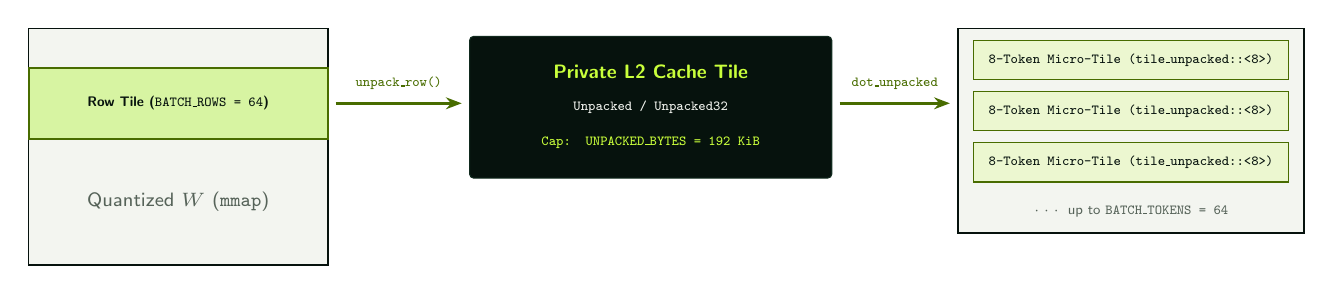
\begin{tikzpicture}[x=1mm, y=1mm]
    % Left: Quantized Matrix W
    \fill[swzBone, draw=swzInk, line width=0.6pt] (0, 0) rectangle (38, 30);
    \fill[swzGainHi, draw=swzOlive, line width=0.7pt] (0, 16) rectangle (38, 25);
    \node[font=\sffamily\bfseries\tiny, text=swzInk] at (19, 20.5) {Row Tile (\texttt{BATCH\_ROWS = 64})};
    \node[font=\sffamily\scriptsize, text=swzMuted] at (19, 8) {Quantized $W$ (\texttt{mmap})};

    % Arrow 1: Unpack once into L2
    \draw[-{Stealth[length=2mm]}, swzOlive, line width=0.9pt] (39, 20.5) -- (55, 20.5);
    \node[above, font=\ttfamily\tiny, text=swzOlive] at (47, 21) {unpack\_row()};

    % Middle: L2 Unpacked Buffer
    \fill[swzInk, draw=swzDark, rounded corners=1.5pt] (56, 11) rectangle (102, 29);
    \node[font=\sffamily\bfseries\scriptsize, text=swzLime] at (79, 24.5) {Private L2 Cache Tile};
    \node[font=\ttfamily\tiny, text=swzBone] at (79, 20) {Unpacked / Unpacked32};
    \node[font=\ttfamily\tiny, text=swzLime] at (79, 15.5) {Cap: \texttt{UNPACKED\_BYTES = 192 KiB}};

    % Arrow 2: Broadcast to 8-token AVX2 micro-tiles
    \draw[-{Stealth[length=2mm]}, swzOlive, line width=0.9pt] (103, 20.5) -- (117, 20.5);
    \node[above, font=\ttfamily\tiny, text=swzOlive] at (110, 21) {dot\_unpacked};

    % Right: 64-token Activation Batch
    \fill[swzBone, draw=swzInk, line width=0.6pt] (118, 4) rectangle (162, 30);
    \foreach \t/\y in {0/23.5, 1/17, 2/10.5} {
      \fill[swzGainMid, draw=swzOlive] (120, \y) rectangle (160, \y+5);
      \node[font=\ttfamily\tiny, text=swzInk] at (140, \y+2.5) {8-Token Micro-Tile (\texttt{tile\_unpacked::<8>})};
    }
    \node[font=\sffamily\tiny, text=swzMuted] at (140, 6.8) {$\cdots$ up to \texttt{BATCH\_TOKENS = 64}};
  \end{tikzpicture}
  \caption{Two-level CPU cache-tiling in \texttt{swizzle-cpu/src/matmul.rs}. Quantized weight rows are unpacked once into a $192\text{ KiB}$ L2-resident \texttt{Unpacked} buffer and multiplied across 8-token AVX2 register micro-tiles.}
  \label{fig:cpu_tiling}
\end{figure}

% ==================== SECTION 6: CUDA BACKEND ====================
\section{CUDA Execution Engine: Dynamic Driver API, Planar GEMV, and Swizzled Tensor-Core GEMM}

\code{swizzle-cuda} interacts directly with the NVIDIA Driver API (\code{cuInit}, \code{cuModuleLoadData}, \code{cuLaunchKernel}, \code{cuStreamBeginCapture\_v2}, \code{cuGraphInstantiate}, \code{cuGraphLaunch}) resolved dynamically via \code{libloading} in \code{driver.rs}. At build time, \code{nvcc} compiles \code{kernels.cu} (which includes all 26 \code{.cuh} headers into a single translation unit) into one embedded fatbin containing native SASS machine code for \code{sm\_75} (Turing), \code{sm\_80}/\code{sm\_86} (Ampere), \code{sm\_89} (Ada), \code{sm\_90} (Hopper), and \code{sm\_120} (Blackwell), plus forward-compatible PTX.

\subsection{Cache-Hierarchy Streaming in Planar \texttt{dp4a} GEMV (\texttt{common.cuh})}

During decode ($N \le 16$), weight matrices are dozens to hundreds of megabytes and cannot fit in the GPU's L1 data cache ($128\text{ KiB}$ per SM), whereas the quantized input vector \code{Q8Input \{ qs, ds \}} is only $4\text{--}16\text{ KiB}$ and is read repeatedly by every weight row assigned to that SM. If weights are loaded with default cache policies, streaming weight blocks evict the hot input vector from L1.

In \code{common.cuh}, Swizzle separates memory traffic into two explicit PTX cache policies:
\begin{lstlisting}[language=C++]
// Weights are streamed once per call; evict-first keeps the reused input
// vector resident in L1.
__device__ __forceinline__ Words load_weights(const void* p) {
    const int4 v = __ldcs(static_cast<const int4*>(p));
    return {{v.x, v.y, v.z, v.w}};
}

__device__ __forceinline__ Words load_cached(const void* p) {
    const int4 v = __ldg(static_cast<const int4*>(p));
    return {{v.x, v.y, v.z, v.w}};
}
\end{lstlisting}
Here \code{\_\_ldcs} emits \code{ld.global.cs.v4.s32} (\emph{cache streaming / evict-first}), tagging weight cache lines for immediate eviction after the warp consumes them, while \code{\_\_ldg} emits \code{ld.global.nc.v4.s32}, pinning the input vector \code{x.qs} and scales \code{x.ds} in the read-only L1 texture/constant cache.

\subsection{Bit-Identical \texttt{dp4a} and Tensor-Core \texttt{mma.sync} Reductions (\texttt{kquant.cuh})}

For small decode batches ($N$ small), one warp per row computes \code{dp4a} integer dot products (\code{gemv\_kquant.cuh}). When the batch grows (e.g., an 8-token or 16-token speculative tree or Convoy pass on \code{sm\_80+}), \code{gemv\_mma.cuh} switches to integer Tensor Core instructions (\code{mma.sync.aligned.m16n8k32.row.col.s32.s8.s8.s32} for $\text{Q4\_K}/\text{Q5\_K}$ and \code{m16n8k16} for $\text{Q6\_K}$), multiplying 16 weight rows across 8 input vectors simultaneously.

To ensure that switching between \code{dp4a} and \code{mma.sync} never changes a single bit of any logit, \code{kquant.cuh} enforces a shared reduction topology across both kernels:
\begin{enumerate}
  \item \textbf{Round-Robin Block Partitioning (\code{KQ\_SPLIT = 4}):} A weight row's 256-element super-blocks are dealt round-robin across 4 partial sums $v \in \{0, 1, 2, 3\}$, so partial sum $v$ accumulates blocks $b \equiv v \pmod 4$ sequentially using explicit round-to-nearest-even \code{\_\_fadd\_rn} (preventing nvcc from fusing additions into FMA instructions).
  \item \textbf{Exact Sub-Block Term Formula (\code{kq\_term}):} Within each super-block, every scale group (8 sub-blocks of 32 for $\text{Q4\_K}/\text{Q5\_K}$, or 16 runs of 16 for $\text{Q6\_K}$) first forms an exact \code{int32} dot product $q \in \mathbb{Z}$ (which is associative and identical between \code{dp4a} and \code{mma.sync}) and converts it to \code{float} via:
  \begin{equation}
    t_s = \text{fmaf}\!\left(\text{rn}(\text{scale}_s \cdot x_{d,s}),\; \text{float}(q_s),\; -\text{rn}(\text{min}_s \cdot x_{\text{sum},s})\right)
  \end{equation}
  \item \textbf{Compile-Time Balanced Binary Tree (\code{TreeSum<K>}):} The $2^K$ group terms ($2^3=8$ for $\text{Q4\_K}/\text{Q5\_K}$, $2^4=16$ for $\text{Q6\_K}$) are folded into the super-block sum using a balanced binary tree $((t_0 + t_1) + (t_2 + t_3)) + \dots$:
\end{enumerate}
\begin{lstlisting}[language=C++]
template <unsigned K>
struct TreeSum {
    float level[K + 1];
    __device__ __forceinline__ void push(unsigned i, float v) {
        unsigned l = 0;
        for (; i & 1; i >>= 1, ++l) v = __fadd_rn(level[l], v);
        level[l] = v;
    }
    __device__ __forceinline__ float total() const { return level[K]; }
};
\end{lstlisting}
In \code{gemv\_kquant.cuh}, the 8 lanes of a sub-warp exchange their group terms via 3 \code{\_\_shfl\_xor\_sync} steps with distances $1, 2, 4$, which computes the exact same balanced binary tree $((t_0 + t_1) + (t_2 + t_3)) + ((t_4 + t_5) + (t_6 + t_7))$ that \code{TreeSum<3>} computes inside a single lane in \code{gemv\_mma.cuh}.

\subsection{Zero-Padding XOR Shared-Memory Swizzling in Tensor-Core GEMM (\texttt{gemm.cuh})}

For prompt prefill ($N \ge 32$), \code{gemm.cuh} executes double-buffered integer Tensor Core matrix multiplication over stages of \code{GEMM\_K = 128} columns (\code{GEMM\_SUBS = 4} sub-blocks of 32), parameterized across three tile geometries:
\begin{itemize}
  \item \code{GemmTile32 = GemmTile<64, 32, 1, 2>}: $64\text{ rows} \times 32\text{ inputs}$, 4 warps ($128$ threads), 2 blocks/SM, $30,720\text{ B}$ shared memory.
  \item \code{GemmTile64 = GemmTile<64, 64, 2, 2>}: $64\text{ rows} \times 64\text{ inputs}$, 4 warps ($128$ threads), 2 blocks/SM, $40,960\text{ B}$ shared memory.
  \item \code{GemmTile128 = GemmTile<128, 128, 2, 1>}: $128\text{ rows} \times 128\text{ inputs}$, 8 warps ($256$ threads), 1 block/SM, $81,920\text{ B}$ shared memory.
\end{itemize}

Each stage buffer \code{GemmStage<T>} stores unpacked \code{int8} weights \code{w[T::ROWS][128]} and \code{int8} activations \code{x[T::COLS][128]}. NVIDIA GPUs partition shared memory into 32 banks of 4 bytes each, so a 128-byte row spans all 32 banks exactly once (bytes $0..127$ map to banks $0..31$). When a warp executes \code{ldmatrix.sync.aligned.m8n8.x4.shared.b16}, lanes $0..7$ (and $8..15$, $16..23$, $24..31$) supply the starting addresses of 8 consecutive rows $(r_0, r_0+1, \dots, r_0+7)$ at the \emph{same} column byte offset $b = 32s + 16(l/16)$. Without address transformation, all 8 rows at column offset $b$ fall into the exact same 4 banks $\lfloor b/4 \rfloor \dots \lfloor b/4 \rfloor + 3$, causing an \textbf{8-way shared-memory bank conflict} on every Tensor Core load!

Conventional GEMM kernels avoid this by padding every 128-byte row to 144 bytes (\code{w[ROWS][144]}). However, $+16\text{ B}$ padding wastes $12.5\%$ of shared memory, inflating \code{GemmTile128}'s two stages past the hardware shared-memory ceiling of consumer GPUs and breaking 128-bit alignment on odd rows.

\begin{theorem}[Bijective Conflict-Free XOR Shared-Memory Swizzle]
Define the byte-offset permutation in \code{crates/swizzle-cuda/cuda/gemm.cuh}:
\begin{equation}
  \text{gemm\_swizzle}(r, b) = b \oplus \left((r \mathbin{\&} 7) \ll 4\right), \qquad r \in \mathbb{Z}_{\ge 0},\quad b \in \{0, 1, \dots, 127\}
  \label{eq:gemm_swizzle}
\end{equation}
Then:
\begin{enumerate}
  \item \textbf{Row-wise Bijection (Zero Padding):} For any fixed row $r$, $\text{gemm\_swizzle}(r, \cdot)$ is an involution on $\{0, \dots, 127\}$ that preserves alignment mod 16, so 16-byte \code{uint4} / \code{cp.async.cg.shared.global} writes stay contiguous within each 16-byte chunk.
  \item \textbf{Column-wise Bank Disjointness (\texttt{ldmatrix.x4}):} For any fixed logical 16-byte chunk $c = \lfloor b/16 \rfloor \in \{0, \dots, 7\}$ and any 8 consecutive rows $r \in \{8k, 8k+1, \dots, 8k+7\}$, the physical 16-byte chunks $c' = c \oplus (r \mathbin{\&} 7)$ traverse $\{0, 1, \dots, 7\}$ bijectively. Because chunk $c'$ occupies shared-memory banks $\{4c', 4c'+1, 4c'+2, 4c'+3\}$, all 8 rows map to $8 \times 4 = 32$ mutually disjoint banks (\textbf{zero bank conflicts}).
\end{enumerate}
\end{theorem}

\begin{figure}[htbp]
  \centering
  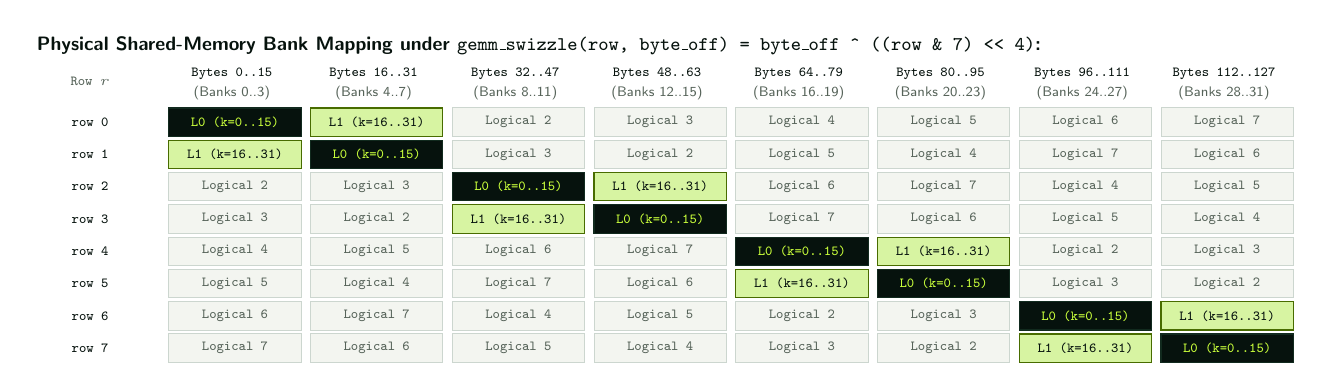
\begin{tikzpicture}[x=1mm, y=1mm]
    \node[anchor=west, font=\sffamily\bfseries\scriptsize, text=swzInk] at (0, 41) {Physical Shared-Memory Bank Mapping under \texttt{gemm\_swizzle(row, byte\_off) = byte\_off \^{} ((row \& 7) << 4)}:};
    % Column headers
    \node[font=\ttfamily\bfseries\tiny, text=swzMuted] at (8, 36.5) {Row $r$};
    \foreach \c in {0,...,7} {
      \pgfmathsetmacro{\x}{18 + \c * 18}
      \pgfmathtruncatemacro{\blo}{\c * 16}
      \pgfmathtruncatemacro{\bhi}{\c * 16 + 15}
      \pgfmathtruncatemacro{\bklo}{\c * 4}
      \pgfmathtruncatemacro{\bkhi}{\c * 4 + 3}
      \node[font=\ttfamily\bfseries\tiny, text=swzInk] at (\x+8, 37.5) {Bytes \blo..\bhi};
      \node[font=\sffamily\tiny, text=swzMuted] at (\x+8, 35) {(Banks \bklo..\bkhi)};
    }
    % Grid of 8 rows x 8 16B chunks
    \foreach \r in {0,...,7} {
      \pgfmathsetmacro{\y}{29.5 - \r * 4.1}
      \node[font=\ttfamily\bfseries\tiny, text=swzInk] at (8, \y+1.8) {row \r};
      \foreach \p in {0,...,7} {
        \pgfmathsetmacro{\x}{18 + \p * 18}
        % Logical chunk L such that L ^ r == p  => L = p ^ r (3-bit bitwise XOR)
        \pgfmathtruncatemacro{\L}{(mod(\p,2)!=mod(\r,2)) + 2*(mod(floor(\p/2),2)!=mod(floor(\r/2),2)) + 4*(mod(floor(\p/4),2)!=mod(floor(\r/4),2))}
        \ifnum\L=0
          \fill[swzInk, draw=swzDark, line width=0.4pt] (\x, \y) rectangle (\x+16.8, \y+3.6);
          \node[font=\ttfamily\bfseries\tiny, text=swzLime] at (\x+8.4, \y+1.8) {L0 (k=0..15)};
        \else
          \ifnum\L=1
            \fill[swzGainHi, draw=swzOlive, line width=0.4pt] (\x, \y) rectangle (\x+16.8, \y+3.6);
            \node[font=\ttfamily\bfseries\tiny, text=swzInk] at (\x+8.4, \y+1.8) {L1 (k=16..31)};
          \else
            \fill[swzBone, draw=swzRule, line width=0.35pt] (\x, \y) rectangle (\x+16.8, \y+3.6);
            \node[font=\ttfamily\tiny, text=swzMuted] at (\x+8.4, \y+1.8) {Logical \L};
          \fi
        \fi
      }
    }
  \end{tikzpicture}
  \caption{Visual proof of conflict-free Tensor Core \texttt{ldmatrix.x4} loads in \texttt{gemm.cuh}. When a warp loads logical chunk \textbf{L0} ($k=0..15$, dark obsidian cells with electric lime text) or \textbf{L1} ($k=16..31$, soft lime cells) across rows $0..7$, the XOR permutation scatters the 8 row accesses diagonally across all 8 physical bank groups (Banks $0..31$), achieving $100\%$ shared-memory bank utilization with zero bytes of padding.}
  \label{fig:xor_swizzle}
\end{figure}

\subsection{IEEE-754 Mantissa Bias Trick for Tensor-Core Accumulation (\texttt{gemm.cuh})}

In \code{gemm\_subs} (\code{gemm.cuh} lines 350--408), each Tensor Core instruction \code{mma\_k32\_from} or \code{mma\_k16\_from} computes $D = A B + C$ where $A$ and $B$ are \code{int8} fragments and $C, D$ are \code{int32}. Standard kernels initialize $C = 0$, receive a signed \code{int32} dot product $d \in [-2^{19}, 2^{19}]$, and execute an expensive \code{I2F} (\code{static\_cast<float>(d)}) conversion instruction for every element of every sub-block before multiplying by the sub-block scale.

Swizzle eliminates the \code{I2F} conversion instructions entirely by passing the constant \code{GEMM\_BIAS\_BITS = 0x4B400000} (which is the IEEE-754 representation of $2^{23} + 2^{22} = 12,582,912.0\text{f}$) as the integer accumulator input $C$ to the \code{mma.sync} instruction itself:
\begin{equation}
  d_{\text{bits}} = \text{mma.sync}(A, B, \texttt{0x4B400000}) = \texttt{0x4B400000} + \sum_{k} a_k b_k
\end{equation}
Because $2^{23} \le 12,582,912 + \sum_k a_k b_k < 2^{24}$, the unit-in-the-last-place (ULP) of a single-precision \code{float} in the exponent range $[2^{23}, 2^{24})$ is \textbf{exactly 1.0}! Adding the signed integer dot product $\sum_k a_k b_k$ directly to the integer bit pattern \code{0x4B400000} inside the Tensor Core's integer adder produces the exact IEEE-754 floating-point bit pattern of $\text{GEMM\_BIAS} + \sum_k a_k b_k$. Reinterpreting the register as a float via zero-cost \code{\_\_int\_as\_float(d[e])} and folding $-\text{GEMM\_BIAS} \cdot \text{scale}_i$ into a precomputed \code{unbias[i]} register merges conversion and scaling into a single hardware FMA:
\begin{lstlisting}[language=C++]
// Adding a small signed integer to GEMM_BIAS_BITS is the bit pattern of
// GEMM_BIAS plus that integer as a float, so __int_as_float reads it
// without an int-to-float conversion and an FMA takes GEMM_BIAS back out.
constexpr int GEMM_BIAS_BITS = 0x4b400000;
constexpr float GEMM_BIAS = 12582912.0f;
// Inside gemm_subs:
for (unsigned i = 0; i < 2 * T::MT; ++i) unbias[i] = -GEMM_BIAS * scale[i];
mma_k32_from(d, a[m][0], a[m][1], a[m][2], a[m][3], b[j][0], b[j][1], GEMM_BIAS_BITS);
acc.v[m][j][e] = fmaf(fmaf(__int_as_float(d[e]), scale[i], unbias[i]), x, v);
\end{lstlisting}
Furthermore, for gated feed-forward layers ($\text{SiLU}(W_{\text{gate}} x) \odot (W_{\text{up}} x)$ or $\text{GELU}(W_{\text{gate}} x) \odot (W_{\text{up}} x)$), \code{gemm.cuh} interleaves gate rows ($R \bmod 16 < 8$) and up-projection rows ($R \bmod 16 \ge 8$) inside the same thread block so each lane holds \emph{both} factors in registers, computes the gated product in \code{gemm\_glu\_out} via shared memory \code{GemmGluTile<T>} (padded by $+4$ floats to avoid bank conflicts), and directly quantizes the output into the next layer's \code{Q8Input} buffer without writing intermediate \code{f32} activations to global VRAM.

% ==================== SECTION 7: VULKAN BACKEND ====================
\section{Vulkan Execution Engine: WGSL-to-SPIR-V via Naga and Subgroup-32 Kernels}

To run accelerated local inference across AMD (RDNA 2/3/4), Intel (Arc / Xe), and NVIDIA GPUs without requiring users to install vendor SDKs, \code{swizzle-vulkan} compiles WebGPU Shading Language (WGSL) compute kernels into SPIR-V bytecode in pure Rust at build time using \code{naga}, and loads the platform Vulkan loader (\code{vulkan-1.dll} or \code{libvulkan.so.1}) dynamically at runtime.

\subsection{Vulkan 1.3 Hardware Capabilities and Unified Memory Selection}

In \code{crates/swizzle-vulkan/src/physical.rs}, \code{DeviceInfo::missing()} checks four mandatory Vulkan 1.3 capabilities required by Swizzle's compute shaders:
\begin{enumerate}
  \item \textbf{Subgroup Size Control \& Arithmetic:} \code{VK\_EXT\_subgroup\_size\_control} with subgroup size 32 so that WGSL subgroup reductions match warp-level reductions on CUDA.
  \item \textbf{Integer Dot Product Intrinsics:} \code{VK\_KHR\_shader\_integer\_dot\_product} (4x8-bit packed mixed-signedness hardware dot product), mapping to \code{dp4a} / \code{v\_dot4\_i32\_i8} instructions.
  \item \textbf{Push Descriptors:} \code{VK\_KHR\_push\_descriptor}, binding buffer descriptors directly into the command buffer without per-step \code{VkDescriptorSet} pool allocations.
  \item \textbf{Smart Heap Placement for iGPUs:} On integrated GPUs (AMD APUs, Intel Arc iGPUs) where the device-local heap is smaller than system memory, \code{swizzle-vulkan} automatically places weight and KV buffers in host-visible, device-accessible system RAM rather than failing allocation or double-buffering across PCIe.
\end{enumerate}

Every \code{VulkanState} records its entire multi-layer decode pass once into a reusable \code{Graph} (\code{VkCommandBuffer} created without \code{ONE\_TIME\_SUBMIT}) that reads the active token count and position from a tiny host-mapped \code{Batch} header buffer (\code{BATCH\_HEADER}), making \textbf{Torque} always-on across all Vulkan GPUs (\code{Tech::switchable\_on} returns \code{false} for \code{Torque} on \code{Device::Vulkan}).

% ==================== SECTION 8: MODEL ARCHITECTURES ====================
\section{Model Architectures: Transformers, Gated DeltaNet, Mamba-2, and LFM 2/3}

In \code{crates/swizzle-models/src/arch/mod.rs}, all supported model families are registered in a single static table \code{FAMILIES}. Loading, architecture support checks (\code{swizzle\_models::supports}), and CLI inspection read exclusively from this declarative table:

\begin{table}[htbp]
  \centering
  \caption{The 10 Model Architecture Families Supported by \texttt{swizzle-models/src/arch/mod.rs}.}
  \label{tab:arch_families}
  \footnotesize
  \begin{tabularx}{\textwidth}{@{}llclX@{}}
    \toprule
    \sffamily\bfseries Family Module & \sffamily\bfseries GGUF Architecture Strings & \sffamily\bfseries Body Kind & \sffamily\bfseries Sequence Mixers & \sffamily\bfseries Special Architectural Mechanics \\
    \midrule
    \code{qwen35} & \code{qwen35}, \code{qwen35moe} & \code{Decoder} & Gated Attention + Gated DeltaNet & Interleaved causal depthwise conv + per-head matrix state $S \in \mathbb{R}^{d_v \times d_k}$ + optional MoE + MTP block. \\
    \code{lfm3} & \code{lfm3}, \code{lfm25} & \code{Decoder} & GQA Attention + ShortConv & Liquid Foundation Model 3 hybrid: gated short causal convolution rings + grouped-query attention. \\
    \code{lfm2} & \code{lfm2}, \code{lfm2moe} & \code{Decoder} & GQA Attention + ShortConv & Dense or routed MoE feed-forward blocks paired with causal \code{ConvWindow} mixers. \\
    \code{transformer} & \code{llama}, \code{qwen2}, \code{qwen3}, \code{qwen3moe}, \code{mistral}, \dots & \code{Decoder} & GQA / MHA Attention & Per-head Q/K RMSNorm (\code{q\_norm}, \code{k\_norm}), YaRN / Linear / NTK RoPE scaling, Dense or MoE FFN. \\
    \code{GEMMA3} & \code{gemma2}, \code{gemma3} & \code{Decoder} & Sliding-Window + Global Attn & $\sqrt{d_{\text{embd}}}$ embedding scale, post-attention \& post-FFN norms, softcap, alternating window sizes. \\
    \code{gemma4} & \code{gemma4} & \code{Decoder} & Hybrid Sliding + Global Attn & Per-layer token embeddings (\code{PerLayer}), value-head RMSNorm (\code{v\_norm}), multimodal 2D/3D grid RoPE. \\
    \code{granite} & \code{granite}, \code{granitemoe}, \code{granitehybrid} & \code{Decoder} & Attention + Mamba-2 & Embedding multiplier, residual multipliers, and output \code{logit\_scale} division. \\
    \code{falcon\_h1} & \code{falcon-h1} & \code{Decoder} & Attention + Mamba-2 SSM & Parallel hybrid layers combining selective state-space scan (\code{Mamba2}) and multi-head attention. \\
    \code{bert} & \code{bert}, \code{nomic-bert}, \code{jina-bert-v2} & \code{Encoder} & Bidirectional Self-Attention & LayerNorm / RMSNorm encoder with mean, CLS, or last-token \code{Pooling} for dense embeddings. \\
    \code{GEMMA\_EMBED} & \code{gemma-embedding} & \code{Bidirectional} & Bidirectional Decoder Stack & Runs decoder layers with causal mask disabled so every token attends to the full sequence. \\
    \bottomrule
  \end{tabularx}
\end{table}

\subsection{Gated Delta-Rule Linear Attention and Chunked Matrix Prefill (\texttt{delta\_net.rs})}

In Qwen 3.5 (\code{qwen35} / \code{qwen35moe}), most layers replace quadratic self-attention with \textbf{Gated DeltaNet} (\code{blocks/delta\_net.rs} and \code{cuda/delta\_net.cuh}). Given hidden state $h_t \in \mathbb{R}^d$, a projection produces queries, keys, and values $(q_t, k_t, v_t)$, which pass through a causal depthwise convolution of \code{conv\_taps} (typically 4) taps followed by $\text{SiLU}$ activation and per-head $L_2$ normalization on $q_t$ and $k_t$. Each value head $h \in \{0, \dots, H_v - 1\}$ maintains a recurrent matrix state $S_t \in \mathbb{R}^{d_v \times d_k}$ updated by the gated delta rule:
\begin{align}
  \gamma_t &= \exp\!\left(a_h \cdot \text{softplus}(\alpha_{t,h} + b_{\text{dt},h})\right), \qquad \beta_{t,h} = \sigma(\tilde{\beta}_{t,h}) \\
  S_t &= \gamma_t S_{t-1} + \beta_{t,h} \left(v_t - \gamma_t S_{t-1} k_t\right) k_t^T, \qquad o_t = S_t q_t
  \label{eq:delta_rule_step}
\end{align}
On CUDA (\code{delta\_net.cuh}), \code{delta\_rule} launches a grid of $(H_v, d_v / 16)$ blocks of 4 warps (128 threads); each warp keeps 4 rows of $S_t$ ($4 \times 128$ floats, 4 values per lane) permanently in registers across all tokens in the batch, updating $S_t$ and computing $o_t = S_t q_t$ with zero global memory traffic for intermediate states.

\begin{proposition}[Chunked WY-Style Triangular Matrix Form of the Gated Delta Rule (\texttt{delta\_chunk.rs})]
When prefilling long prompts ($N \ge \text{CHUNKED\_MIN\_TOKENS} = 32$), stepping Equation~(\ref{eq:delta_rule_step}) token by token is memory-bandwidth-bound on $S_t$. Partition the batch into chunks of $C = 16$ tokens (\code{CHUNK = 16} on AVX2, or \code{PREFILL\_GRID = 32} on CUDA \code{delta\_chunk.cuh}). Let $H = S_0^T \in \mathbb{R}^{d_k \times d_v}$ be the state entering the chunk, and let $G_t = \prod_{j=0}^{t} \gamma_j$ be the cumulative scalar decay within the chunk. Then the 16 rank-1 updates $d_t \in \mathbb{R}^{1 \times d_v}$ stacked as rows of $D \in \mathbb{R}^{C \times d_v}$ satisfy the unit lower-triangular linear system:
\begin{equation}
  (I_C + A) D = \text{diag}(\beta) \left(V - \text{diag}(G) K H\right), \qquad A_{t,j} = \begin{cases} \beta_t (k_t \cdot k_j) \dfrac{G_t}{G_j} & \text{if } j < t \\ 0 & \text{if } j \ge t \end{cases}
  \label{eq:chunked_delta_system}
\end{equation}
Solving $(I_C + A) D$ by forward substitution costs only $O(C^2 d_v)$ operations, after which the chunk outputs $O \in \mathbb{R}^{C \times d_v}$ and final state $H_C \in \mathbb{R}^{d_k \times d_v}$ are computed via matrix-matrix products:
\begin{equation}
  O_t = G_t q_t H + \sum_{j \le t} (q_t \cdot k_j) \frac{G_t}{G_j} d_j, \qquad H_C = G_{C-1} H + \sum_{j=0}^{C-1} \frac{G_{C-1}}{G_j} k_j^T d_j
\end{equation}
\end{proposition}
In \code{delta\_chunk.rs}, Swizzle stacks keys $K$ and queries $Q$ into a single $2C \times d_k$ matrix \code{kq} so one matrix product \code{kq * H} computes both $K H$ and $Q H$ simultaneously.

\subsection{Journaled Checkpointing for Recurrent Speculative Rollback (\texttt{DeltaNetState} \& \texttt{Mamba2State})}

A major obstacle to running speculative decoding (\textbf{RAD-1}) on hybrid recurrent models (Qwen 3.5, LFM 2/3, Falcon-H1) is state rollback: whereas an attention KV cache is indexed by position and rolls back by simply decrementing the sequence cursor, a recurrent state $S_t$ overwrites $S_{t-1}$ in place. Cloning the entire multi-megabyte recurrent state before every token in a draft tree would destroy memory bandwidth.

\begin{decisionbox}{Coding Decision: Checkpoint + Forward-Replay Journals for Recurrent Mixers}
In \code{DeltaNetState} (\code{delta\_net.rs}), \code{Mamba2State} (\code{mamba2.rs}), and \code{cuda/delta\_net.cuh}:
\begin{enumerate}
  \item When \code{checkpoint()} is called before verifying a speculative draft of $1 + k$ tokens, the state records a snapshot of $S_{\text{ckpt}}$ (or leaves \code{s\_in} untouched on GPU while writing to \code{s\_out}) and opens a compact \code{Journal} holding the normalized per-token recurrence inputs $(k_t, v_t, \gamma_t, \beta_t)$ (for DeltaNet) or $(\text{xbc}_t, \Delta t_t)$ (for Mamba-2).
  \item After verification accepts a subset path $\pi = [0, r_1, \dots, r_m]$ of the draft, \code{rollback\_rows} restores $S_{\text{ckpt}}$ and replays \emph{only the recurrence kernel} (\code{delta\_rule} with \code{out = nullptr}) over the $m$ accepted journal rows. The expensive $O(d^2)$ linear projections (\code{qkv}, \code{z}, \code{in\_proj}, \code{out}) are \textbf{never re-executed}.
\end{enumerate}
\end{decisionbox}

\subsection{Dual-Half Precision FlashAttention and Chunk-64 Decode Attention}

In \code{cuda/attention.cuh}, decode attention splits the KV cache into fixed chunks of \code{ATTN\_CHUNK = 64} positions starting at exact multiples of 64, regardless of how many tokens share the batch, and merges chunk log-sum-exp statistics in \code{attn\_combine}. For large prefill batches, \code{cuda/attention\_flash.cuh} implements a custom Tensor Core FlashAttention kernel (\code{FLASH\_Q = 64} queries per 4-warp block, \code{FLASH\_PAD = 8} \code{f16} elements of shared-memory bank padding). To prevent \code{f16} Tensor Core precision loss on high-magnitude queries or attention weights without giving up \code{f16} Tensor Core speed, \code{attention\_flash.cuh} decomposes each \code{f32} query $q$ (and softmax weight) into a pair of \code{f16} numbers $(q_{\text{hi}}, q_{\text{lo}})$ where $q_{\text{hi}} = \text{f16}(q)$ and $q_{\text{lo}} = \text{f16}(q - q_{\text{hi}})$, executing two \code{mma} passes whose sum recovers full \code{f32} inner-product accuracy!

% ==================== SECTION 9: SHORTLIST ====================
\section{Shortlist: Exact Error-Bounded $\text{Q4\_K}$ Vocabulary Screening}

In modern small and medium language models with large multilingual vocabularies, such as \code{Qwen3-0.6B} ($V = 151,936$, $d = 1024$) or Gemma ($V = 256,000$), the output head matrix $W_{\text{head}} \in \mathbb{R}^{V \times d}$ accounts for $20\%\text{--}35\%$ of all parameter bytes read on every decode step. Worse, GGUF models frequently quantize $W_{\text{head}}$ at higher precision ($\text{Q8\_0}$ at $8.5\text{ bits/weight}$ or $\text{Q6\_K}$ at $6.5625\text{ bits/weight}$) than interior layers to preserve perplexity. Yet greedy decoding, top-$k$ sampling, and speculative verification only depend on the \textbf{top $k$ highest logits} of each row!

Naively replacing $W_{\text{head}}$ with a lower-bit approximation alters token choices whenever two candidate logits are close. \textbf{Shortlist} (\code{crates/swizzle-models/src/head/mod.rs}, \code{compact.rs}, and \code{crates/swizzle-cuda/cuda/shortlist.cuh}) solves this exactly: it screens all $V$ rows using an in-memory $\text{Q4\_K}$ copy ($4.5\text{ bits/weight}$, reducing footprint by $31.4\%$ vs.\ $\text{Q6\_K}$ and $47.1\%$ vs.\ $\text{Q8\_0}$) and computes a \textbf{rigorous mathematical upper bound} on every row's exact logit, evaluating the true $\text{Q8\_0}/\text{Q6\_K}$ head \emph{only} on rows whose upper bound can reach the $k$-th best exact logit floor.

\subsection{Mathematical Derivation of the Three-Term Cauchy-Schwarz + IEEE-754 Bound}

Let $w_r \in \mathbb{R}^d$ be the exact dequantized $r$-th row of the output head $W_{\text{head}}$ ($\text{Q8\_0}$ or $\text{Q6\_K}$), and let $c_r \in \mathbb{R}^d$ be the dequantized $r$-th row of its $\text{Q4\_K}$ copy constructed at model load time by \code{compact::build}. During inference on an activation vector $x \in \mathbb{R}^d$, the head kernel multiplies $w_r$ by its quantized activation vector $x_h \in \mathbb{R}^d$ (quantized in 32-element $\text{Q8}$ blocks for $\text{Q8\_0}$ or 256-element $\text{Q8\_K}$ blocks for $\text{Q6\_K}$), producing the floating-point hardware product $\widehat{w_r \cdot x_h}$, while the $\text{Q4\_K}$ screening kernel multiplies $c_r$ by the $\text{Q8\_K}$-quantized activation $x_c \in \mathbb{R}^d$, producing $\widehat{c_r \cdot x_c}$.

\begin{theorem}[Exact Shortlist Screening Upper Bound (\texttt{head/compact.rs})]
Decompose the difference between the true hardware dot product $\widehat{w_r \cdot x_h}$ and the screening hardware dot product $\widehat{c_r \cdot x_c}$ via the triangle and Cauchy-Schwarz inequalities:
\begin{align}
  \widehat{w_r \cdot x_h} - \widehat{c_r \cdot x_c}
  &= \underbrace{\left(\widehat{w_r \cdot x_h} - w_r \cdot x_h\right)}_{\text{Head FP32 rounding}}
   + \underbrace{(w_r - c_r) \cdot x_h}_{\text{Quantization residual}}
   + \underbrace{c_r \cdot (x_h - x_c)}_{\text{Activation quant mismatch}}
   + \underbrace{\left(c_r \cdot x_c - \widehat{c_r \cdot x_c}\right)}_{\text{Copy FP32 rounding}}
\end{align}
Both the head kernel and the $\text{Q4\_K}$ kernel compute exact integer block sums and fold them into \code{f32} with fewer than $d + 8$ floating-point roundings on any execution path. With IEEE-754 round-to-nearest unit roundoff $u = 2^{-24}$ and safety factor $2\times$ covering scale conversions and bound arithmetic, define the rounding slack:
\begin{equation}
  \delta_{\text{slack}} = (d + 8) \cdot 2^{-23}
\end{equation}
For each vocabulary row $r \in \{0, \dots, V-1\}$, precompute at model load time three directed-rounded (\code{f32::next\_up()}) row radii:
\begin{align}
  R_{\text{head}}[r] &= \text{round\_up}\!\left(\|w_r - c_r\|_2 + \delta_{\text{slack}} \|w_r\|_2\right) \\
  R_{\text{copy}}[r] &= \text{round\_up}\!\left(\|c_r\|_2\right) \\
  R_{\text{spread}}[r] &= \text{round\_up}\!\left(\sqrt{\sum_{b=0}^{d/256 - 1} \sum_{i \in b} \left(d_b sc_{b,i} q_{b,i} + d_{\min,b} m_{b,i}\right)^2}\right)
\end{align}
where $R_{\text{spread}}[r]$ measures the $L_2$ norm of the unsigned scaled $\text{Q4\_K}$ terms and offsets before subtraction, which is the exact magnitude the $\text{Q4\_K}$ kernel's \code{f32} rounding acts upon. Then for any token $t$, with activation norms $s_h = \|x_h\|_2$, $s_{\text{gap}} = \|x_h - x_c\|_2$, and $s_c = \delta_{\text{slack}} \|x_c\|_2$, the exact hardware logit $\widehat{w_r \cdot x_h}$ is strictly bounded above by:
\begin{equation}
  \widehat{w_r \cdot x_h} \;\le\; \text{Bound}(r, t) \;\triangleq\; \widehat{c_r \cdot x_c} + R_{\text{head}}[r]\, s_h + R_{\text{copy}}[r]\, s_{\text{gap}} + R_{\text{spread}}[r]\, s_c
  \label{eq:shortlist_bound}
\end{equation}
\end{theorem}

\begin{figure}[htbp]
  \centering
  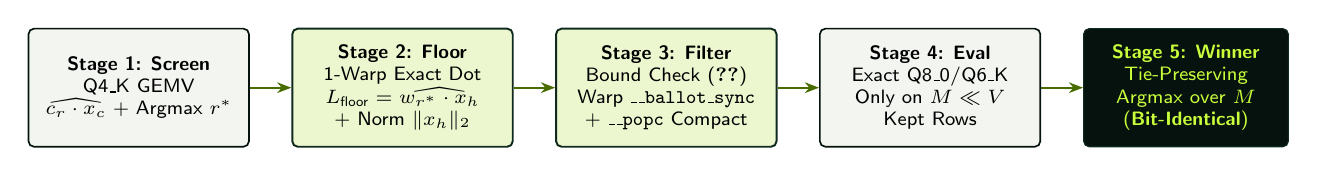
\begin{tikzpicture}[
    stage/.style={draw=swzInk, line width=0.6pt, fill=swzBone, rounded corners=2pt, minimum width=28mm, minimum height=15mm, inner sep=4pt, align=center, font=\sffamily\scriptsize},
    gpustage/.style={draw=swzDark, line width=0.7pt, fill=swzGainMid, rounded corners=2pt, minimum width=28mm, minimum height=15mm, inner sep=4pt, align=center, font=\sffamily\scriptsize},
    arr/.style={-{Stealth[length=1.8mm]}, draw=swzOlive, line width=0.8pt}
  ]
    \node[stage] (s1) at (0,0) {\textbf{Stage 1: Screen}\\$\text{Q4\_K}$ GEMV\\$\widehat{c_r \cdot x_c}$ + Argmax $r^*$};
    \node[gpustage] (s2) at (3.35,0) {\textbf{Stage 2: Floor}\\1-Warp Exact Dot\\$L_{\text{floor}} = \widehat{w_{r^*} \cdot x_h}$\\+ Norm $\|x_h\|_2$};
    \node[gpustage] (s3) at (6.7,0) {\textbf{Stage 3: Filter}\\Bound Check (\ref{eq:shortlist_bound})\\Warp \texttt{\_\_ballot\_sync}\\+ \texttt{\_\_popc} Compact};
    \node[stage] (s4) at (10.05,0) {\textbf{Stage 4: Eval}\\Exact $\text{Q8\_0}/\text{Q6\_K}$\\Only on $M \ll V$\\Kept Rows};
    \node[fill=swzInk, draw=swzDark, rounded corners=2pt, minimum width=26mm, minimum height=15mm, inner sep=4pt, align=center, font=\sffamily\scriptsize, text=swzLime] (s5) at (13.3,0) {\textbf{Stage 5: Winner}\\Tie-Preserving\\Argmax over $M$\\(\textbf{Bit-Identical})};

    \draw[arr] (s1) -- (s2);
    \draw[arr] (s2) -- (s3);
    \draw[arr] (s3) -- (s4);
    \draw[arr] (s4) -- (s5);
  \end{tikzpicture}
  \caption{Five-stage zero-host-synchronization GPU Shortlist pipeline in \texttt{crates/swizzle-cuda/src/shortlist.rs} and \texttt{shortlist.cuh}. All counters (\texttt{d\_floor}, \texttt{d\_norm}, \texttt{d\_count}) remain in device memory so the entire 5-kernel sequence is capturable inside a \textbf{Torque} CUDA graph.}
  \label{fig:shortlist_pipeline}
\end{figure}

\subsection{Zero-Sync Warp-Aggregated Compaction on CUDA (\texttt{shortlist.cuh})}

On CUDA (\code{shortlist.cuh}), when screening for greedy decoding where both the $\text{Q8\_0}$ or $\text{Q6\_K}$ head and the $\text{Q4\_K}$ copy read the exact same 32-element quantized \code{Q8Input} ($x_h = x_c$, so $s_{\text{gap}} = \|x_h - x_c\|_2 = 0$), Equation~(\ref{eq:shortlist_bound}) simplifies to two fused multiply-adds per row using interleaved \code{[head\_radius, spread\_radius]} pairs (\code{float2 rad = radii[r]}):
\begin{lstlisting}[language=C++]
const float2 rad = __ldg(radii + r);
const float approx_v = approx[r];
const float err = __fmaf_ru(rad.x, norm, __fmul_ru(rad.y, slack * norm));
const float ub = __fadd_ru(approx_v, err);
const bool keep = (r == best_r) || !(ub < floor_v);

const unsigned mask = __ballot_sync(FULL_MASK, keep);
if (mask == 0) return;
const unsigned lane = threadIdx.x % WARP;
const unsigned warp_cnt = __popc(mask);
unsigned base = 0;
if (lane == 0) base = atomicAdd(d_count, warp_cnt);
base = __shfl_sync(FULL_MASK, base, 0);
if (keep) {
    const unsigned offset = __popc(mask & ((1u << lane) - 1u));
    kept_idx[base + offset] = r;
}
\end{lstlisting}
Notice two crucial hardware engineering details in \code{shortlist\_filter}:
\begin{enumerate}
  \item \textbf{Directed Rounding Upward in Hardware (\code{\_\_fmaf\_ru}, \code{\_\_fadd\_ru}):} The upper bound is computed using IEEE-754 round-toward-$+\infty$ PTX instructions (\code{fma.rp.f32}, \code{add.rp.f32}), guaranteeing that floating-point evaluation of the bound itself can never underestimate $\text{Bound}(r, t)$.
  \item \textbf{Warp-Ballot Atomic Compaction:} Rather than issuing up to 32 conflicting global \code{atomicAdd} calls per warp, \code{\_\_ballot\_sync(FULL\_MASK, keep)} collects the 32-bit predicate mask across the warp, lane 0 executes a \emph{single} \code{atomicAdd(d\_count, \_\_popc(mask))}, broadcasts \code{base} via \code{\_\_shfl\_sync}, and each surviving lane writes its row index to \code{base + \_\_popc(mask \& ((1u << lane) - 1u))}.
\end{enumerate}
On the CPU (\code{head/mod.rs}), if the number of surviving rows $M = \text{kept\_rows.len()}$ exceeds $\frac{1}{3} V$ (where indexed gather + screening would cost at least as much as a single contiguous pass), Shortlist falls back transparently; otherwise \code{matmul\_indexed\_prepared} evaluates only the $M$ surviving rows.

% ==================== SECTION 10: RAD-1 SPECULATIVE DECODING ====================
\section{RAD-1: Lossless Ensemble Speculative Decoding}

Autoregressive generation is memory-bandwidth-bound because reading $B_{\text{weights}}$ bytes from RAM or VRAM produces only 1 token. If a lightweight \textbf{Drafter} proposes a sequence (or tree) of $k$ candidate tokens $[\hat{t}_1, \dots, \hat{t}_k]$ at negligible cost, the target model can evaluate the current token $t_0$ together with all $k$ draft tokens in a \textbf{single batched forward pass} of width $1 + k$. When $a \in \{0, \dots, k\}$ draft tokens are accepted, the pass yields $1 + a$ exact tokens for the cost of one weight read!

However, single-source speculative decoders fail across diverse workloads:
\begin{itemize}
  \item $n$-gram context lookup is virtually free and achieves $80\%+$ acceptance when editing code, refactoring functions, or quoting documents, but proposes 0 tokens on novel creative prose.
  \item Neural Multi-Token Prediction (MTP) heads propose tokens on novel prose, but their draft length is short ($1\text{--}2$ tokens) and they miss long verbatim spans from earlier files in the session.
\end{itemize}

\textbf{RAD-1} (\code{crates/swizzle-models/src/speculative/}) solves this by combining three complementary drafters inside an online score-weighted tree ensemble (\code{Ensemble<D>}), paired with adaptive draft-length and exponential-backoff pause control.

\subsection{The Three Drafter Sources: \texttt{Lookup}, \texttt{SessionIndex} SAM, and \texttt{MtpDrafter}}

\subsubsection{1. Prompt Suffix Lookup (\texttt{speculative/lookup.rs})}
\code{Lookup} scans the current sequence's token slice \code{context} backward for the most recent earlier occurrence of the longest suffix of length $g \in [\text{min\_ngram}, \text{max\_ngram}]$ (default $g \in [2..=4]$) and proposes the up to \code{limit} tokens that immediately followed that match. Its cost is sub-microsecond and requires zero extra memory.

\subsubsection{2. Linear-Time Suffix Automaton Over the Whole Session (\texttt{speculative/session.rs})}
In multi-turn coding sessions or agentic workflows, the user often edits a file that appeared in an earlier turn or was loaded into the workspace. \code{SessionIndex} maintains an online \textbf{Suffix Automaton (SAM)} over up to \code{capacity = 1 << 18} ($262,144$) tokens observed across the entire session, using a custom rotate-multiply \code{FxHasher} (\code{0x517cc1b727220a95}) for $(u32, u32)$ state-token transitions and keeping memory near $\sim 100\text{ bytes/token}$:
\begin{lstlisting}[language=Rust]
struct Node {
    len: u32,       // Length of the longest string the state stands for.
    link: u32,      // Suffix link: longest suffix ending in more places.
    first_out: u32, // Head of transition list in `out` for cloning states.
    recent: u32,    // Latest end position of the state's strings.
    earlier: u32,   // Second-latest end position (used when `recent` is the current tail).
}
\end{lstlisting}
Appending each observed token to the suffix automaton runs in $O(1)$ amortized time and updates the \code{recent} and \code{earlier} end-positions up to suffix link depth \code{RECENCY\_DEPTH = 64}. When proposing a draft, \code{SessionIndex} walks the automaton over the context suffix to find the longest match of length $\ge \text{min\_match} = 3$ and returns the tokens that followed its most recent earlier occurrence.

\subsubsection{3. Neural Multi-Token Prediction Head (\texttt{speculative/mtp.rs})}
For models that ship with a native Multi-Token Prediction block in GGUF (such as Qwen 3.5), \code{MtpDrafter} feeds the target model's final normalized hidden state $h_t \in \mathbb{R}^d$ and chosen token $t_{t+1}$ into the MTP block to predict $\hat{t}_{t+2}$ (and chains on its own output up to \code{depth = 2}, restricting the draft head to the first \code{draft\_vocab = 32768} frequent vocabulary rows for speed), after first checking a fast $g \in [3..=4]$ context lookup.

\begin{figure}[htbp]
  \centering
  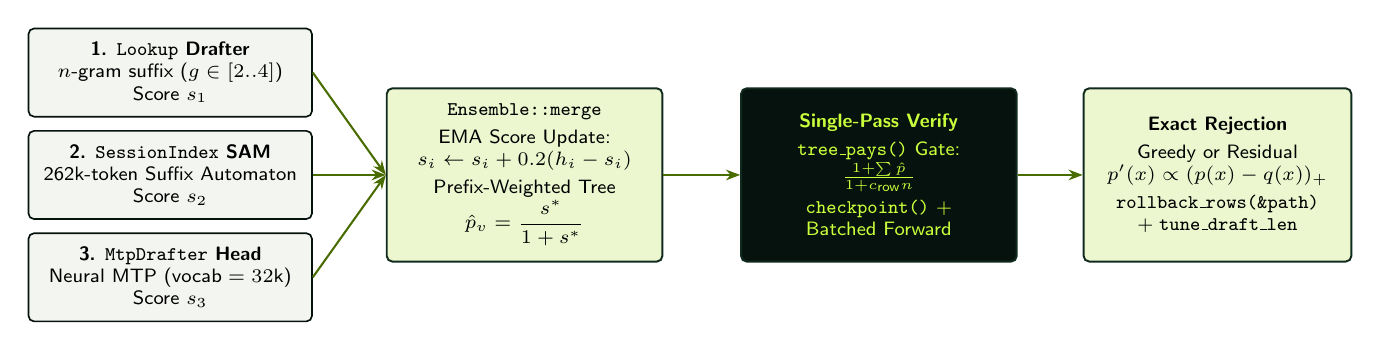
\begin{tikzpicture}[
    box/.style={draw=swzInk, line width=0.6pt, fill=swzBone, rounded corners=2pt, inner sep=5pt, font=\sffamily\scriptsize, align=center},
    gbox/.style={draw=swzDark, line width=0.7pt, fill=swzGainMid, rounded corners=2pt, inner sep=5pt, font=\sffamily\scriptsize, align=center},
    darkbox/.style={draw=swzDark, line width=0.7pt, fill=swzInk, rounded corners=2pt, inner sep=5pt, font=\sffamily\scriptsize, text=swzLime, align=center},
    arr/.style={-{Stealth[length=1.8mm]}, draw=swzOlive, line width=0.75pt}
  ]
    % 3 Drafters
    \node[box, minimum width=36mm, minimum height=11mm] (d1) at (0, 1.3) {\textbf{1. \texttt{Lookup} Drafter}\\$n$-gram suffix ($g \in [2..4]$)\\Score $s_1$};
    \node[box, minimum width=36mm, minimum height=11mm] (d2) at (0, 0) {\textbf{2. \texttt{SessionIndex} SAM}\\262k-token Suffix Automaton\\Score $s_2$};
    \node[box, minimum width=36mm, minimum height=11mm] (d3) at (0, -1.3) {\textbf{3. \texttt{MtpDrafter} Head}\\Neural MTP ($\text{vocab}=32\text{k}$)\\Score $s_3$};

    % Ensemble Merger
    \node[gbox, minimum width=35mm, minimum height=22mm] (ens) at (4.5, 0) {\textbf{\texttt{Ensemble::merge}}\\[2pt]EMA Score Update:\\$s_i \leftarrow s_i + 0.2(h_i - s_i)$\\[2pt]Prefix-Weighted Tree\\$\hat{p}_v = \dfrac{s^*}{1 + s^*}$};

    % Cost Gate & Batch
    \node[darkbox, minimum width=35mm, minimum height=22mm] (ver) at (9.0, 0) {\textbf{Single-Pass Verify}\\[2pt]\texttt{tree\_pays()} Gate:\\$\frac{1 + \sum \hat{p}}{1 + c_{\text{row}} n}$\\[2pt]\texttt{checkpoint()} +\\Batched Forward};

    % Rollback & Policy
    \node[gbox, minimum width=34mm, minimum height=22mm] (pol) at (13.3, 0) {\textbf{Exact Rejection}\\[2pt]Greedy or Residual\\$p'(x) \propto (p(x) - q(x))_+$\\[2pt]\texttt{rollback\_rows(\&path)}\\+\;\texttt{tune\_draft\_len}};

    \draw[arr] (d1.east) -- (ens.west);
    \draw[arr] (d2.east) -- (ens.west);
    \draw[arr] (d3.east) -- (ens.west);
    \draw[arr] (ens.east) -- (ver.west);
    \draw[arr] (ver.east) -- (pol.west);
  \end{tikzpicture}
  \caption{Architecture of the \textbf{RAD-1} speculative decoding subsystem in \texttt{swizzle-models/src/speculative/}. Every drafter is scored against actual generated tokens whether or not its branch was selected.}
  \label{fig:rad1_architecture}
\end{figure}

\subsection{Ensemble Tree Merging, Counterfactual Scoring, and Adaptive Pauses (\texttt{ensemble.rs})}

In \code{Ensemble<D>} (\code{ensemble.rs}), every source $i$ maintains an exponential moving average score $s_i$ initialized to $1.0$ with learning rate \code{RATE = 0.2}. Crucially, on the next step, each source's previous draft is compared against the tokens the target model \emph{actually produced}, regardless of whether source $i$'s branch was the one verified:
\begin{equation}
  s_i \leftarrow s_i + 0.2 \left(\text{hits}_i - s_i\right), \qquad \text{hits}_i = \max\left\{m \;\middle|\; \hat{t}_{i, 1..m} = t_{\text{actual}, 1..m}\right\}
\end{equation}
Thus a source that was outvoted never needs to waste a verification pass to prove that it has started matching the text! When merging branches into a token tree (\code{merge}), shared prefixes sum the weights $s_i$ of all sources proposing them, children are sorted heaviest-first so the leading chain is the highest-weight path, and a node whose best source through it has mean run length $s^*$ is assigned per-token acceptance probability $\hat{p} = \frac{s^*}{1 + s^*}$ (the exact geometric-distribution hazard rate corresponding to mean run length $s^*$).

Before verifying a branching tree versus its leading chain, \code{Decoder::tree\_pays} evaluates the expected tokens per unit of hardware compute cost:
\begin{equation}
  \text{Rate}(n) = \frac{1 + \sum_{j=1}^{n} \hat{p}_j}{1 + c_{\text{row}} \cdot n}
\end{equation}
After each verification step (\code{tune\_draft\_len}), if all drafted tokens were accepted ($\text{accepted} == \text{drafted}$), \code{draft\_len} doubles up to \code{max\_draft}; otherwise it resets immediately to $\text{accepted} + 1$. If zero draft tokens were accepted ($\text{accepted} == 0$), drafting pauses with exponential backoff $\text{pause} = \min(2 \cdot \text{pause}, \text{max\_pause})$ so the runtime never wastes wide passes on unpredictable text.

\subsection{Proof of Exact Distribution Preservation under Greedy and Sampled Decoding}

\begin{theorem}[Lossless Greedy and Residual Rejection Sampling (\texttt{speculative/mod.rs})]
Let $p(\cdot \mid x_{<t})$ be the target model's probability distribution at step $t$ after applying temperature, top-$k$, top-$p$, min-$p$, typical, and DRY/repetition penalties, and let $\hat{t}$ be the deterministic draft token proposed by the drafter ($q(\hat{t}) = 1$, $q(x) = 0$ for $x \neq \hat{t}$):
\begin{enumerate}
  \item \textbf{Greedy Policy:} Verification chooses $t^* = \arg\max_x \text{logit}(x)$ using the exact same \code{Policy::choose} function on row $r$ of the batch. By the Swizzle Batch-Invariance Contract, $\text{logit}(x)$ at row $r$ equals single-token $\text{logit}(x)$ bit-for-bit. The draft $\hat{t}$ is accepted iff $t^* = \hat{t}$, and the first rejected row emits $t^*$ directly. Hence the output sequence is token-for-token identical to non-speculative greedy decoding.
  \item \textbf{Stochastic Sampling Policy (\texttt{Sampler}):} Using one pseudo-random uniform draw $u \sim \text{Uniform}(0, 1)$ per position in identical sequential order, accept $\hat{t}$ with probability $p(\hat{t})$. Upon rejection (which occurs with probability $1 - p(\hat{t})$), draw $t^*$ from the renormalized distribution $p_{\setminus \hat{t}}(x) = \frac{p(x)}{1 - p(\hat{t})}$ for $x \neq \hat{t}$. Then for every token $x \in \mathcal{V}$, the marginal probability of emitting $x$ is:
  \begin{equation}
    \mathbb{P}(\text{emit } x) = \begin{cases} p(\hat{t}) & \text{if } x = \hat{t} \\[4pt] (1 - p(\hat{t})) \cdot \dfrac{p(x)}{1 - p(\hat{t})} = p(x) & \text{if } x \neq \hat{t} \end{cases}
  \end{equation}
  matching $p(x)$ identically while consuming exactly one PRNG draw per position.
\end{enumerate}
\end{theorem}

% ==================== SECTION 11: WARM START & ZERO WAIT ====================
\section{Warm Start and Zero Wait: Prefix State Caching and Keystroke Prefill}

In interactive chat sessions, coding assistants, and tool-using agents, $80\%\text{--}99\%$ of each request's prompt tokens (system instructions, JSON tool schemas, and prior conversation turns) are identical to the preceding request. Re-computing prefill over those prefix tokens wastes seconds of TTFT and tens of watts of GPU/CPU power.

\subsection{Warm Start: Two-Tier Memory/Disk Prefix Cache with Recurrent Grid Marks (\texttt{warm/mod.rs})}

\code{Warm<'m>} (\code{crates/swizzle-models/src/warm/mod.rs}) caches exact post-prefill \code{State} objects and their final next-token \code{logits: Vec<f32>} in memory (default budget \code{WARM\_MEMORY = 1 << 30}, $1\text{ GiB}$) and asynchronously on disk (default budget \code{WARM\_DISK = 2 << 30}, $2\text{ GiB}$).

While pure Transformer KV caches can be truncated in place to \emph{any} prefix length $L_{\text{hit}}$, hybrid models with recurrent layers (\code{DeltaNet}, \code{Mamba2}, \code{ShortConv}) overwrite their state at each token. To make recurrent and hybrid models prefix-cacheable without storing a checkpoint at every single token, \code{Warm} introduces \textbf{adaptive grid marking}:
\begin{enumerate}
  \item \textbf{Adaptive Checkpoint Grid (\code{GRID = 256}, \code{MAX\_GRID = 8192}):} For any model with recurrent layers, \code{Warm} computes a mark stride that is a multiple of $256$ tokens (scaling up toward $8192$ if a recurrent snapshot is large relative to per-token attention KV growth). During prefill, \code{Warm::run} calls \code{runner.mark(\&mut state)} at every grid multiple \emph{and} at the exact \code{branch} point where the new prompt diverges from existing cache entries.
  \item \textbf{Batch-Boundary Alignment (\code{Warm::aligned(PREFILL\_GRID)}):} On CUDA, prefill kernels sum terms in chunks aligned to \code{PREFILL\_GRID = 32}. \code{Warm::aligned(32)} constrains all cache restores and batch cuts to multiples of 32 tokens (unless the entire prompt is an exact cache hit), guaranteeing that a warm prefill produces the \textbf{exact same floating-point bits} as a cold prefill!
  \item \textbf{Cost-Benefit Admission \& Restore Gate (\code{worth\_keeping}):} Restoring or saving a state of $B_{\text{state}}$ bytes is only faster than re-running $L_{\text{hit}}$ tokens if the prefill time saved exceeds the memory/disk transfer cost. \code{Warm} continuously measures the model's prefill rate $r_{\text{prefill}}$ (seconds/token), memory restore rate $r_{\text{restore}}$ (seconds/byte, initialized to $1/(8\times 10^9)\text{ s/B}$), and disk load rate $r_{\text{load}}$ (initialized to $1/(5\times 10^8)\text{ s/B}$), admitting a state to the cache if and only if:
  \begin{equation}
    L_{\text{tokens}} \cdot r_{\text{prefill}} \;\ge\; 2.0 \cdot B_{\text{state}} \cdot r_{\text{restore}}
    \label{eq:warm_worth_keeping}
  \end{equation}
  \item \textbf{Atomic Background \code{.kwarm} Persistence (\code{warm/disk.rs}):} Disk entries are keyed by a 64-bit hash of $(\text{model\_id}, \text{tokens})$, magic header \code{b"KNWARM\textbackslash 0\textbackslash 0"} (\code{VERSION = 1}), written on a background thread to \code{<hash>.<pid>.kwarm-tmp} and atomically renamed to \code{<hash>.kwarm}. Entries whose token prefix is a strict prefix of a newly saved entry (\code{meta.covers(\&f.meta)}) are automatically pruned from both RAM and disk.
\end{enumerate}

\subsection{Zero Wait: Live Keystroke Speculative Prefill (\texttt{swizzle-cli/src/ahead.rs})}

Even with Warm Start caching prior conversation turns, a user typing a new 60-word prompt in \code{swizzle-rt chat} takes $8\text{--}15\text{ seconds}$ at human typing speeds ($40\text{--}70\text{ WPM}$), during which the local CPU and GPU sit completely idle.

\begin{decisionbox}{Coding Decision: Condvar-Driven Live Keystroke Prefill (\texttt{ahead.rs})}
In \code{swizzle-cli/src/ahead.rs}, \code{Typing} shares a mutex-protected \code{Draft \{ messages, options, lines, line, version, done \}} and a \code{Condvar} between the terminal readline thread and a dedicated background worker executing \code{Typing::run(engine)}:
\begin{enumerate}
  \item On every keystroke that modifies the current input line, \code{Typing::line(line)} copies the string, increments \code{d.version += 1}, and signals \code{self.changed.notify\_one()}.
  \item The background thread wakes, formats the full chat template with the user's partial message \code{format!("\{\}\{\}", d.lines, d.line)}, and calls \code{engine.warm(\&Request \{ prompt: Prompt::Chat(messages), .. \})}.
  \item Each background \code{engine.warm} call resumes from the previous keystroke's cached Warm Start state and prefills only the newly typed tokens! By the time the user presses \textbf{Enter}, up to $95\%\text{--}100\%$ of the prompt is already prefilled in the Warm Start cache, collapsing perceived TTFT to near zero.
\end{enumerate}
\end{decisionbox}

\begin{figure}[htbp]
  \centering
  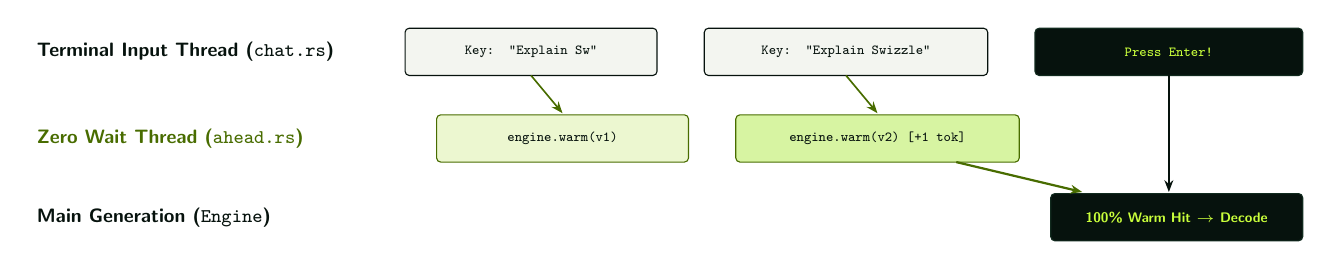
\begin{tikzpicture}[x=1mm, y=1mm]
    % Terminal Thread
    \node[anchor=west, font=\sffamily\bfseries\scriptsize, text=swzInk] at (0, 22) {Terminal Input Thread (\texttt{chat.rs})};
    \fill[swzBone, draw=swzInk, rounded corners=1.5pt] (48, 19) rectangle (80, 25);
    \node[font=\ttfamily\tiny, text=swzInk] at (64, 22) {Key: "Explain Sw"};
    \fill[swzBone, draw=swzInk, rounded corners=1.5pt] (86, 19) rectangle (122, 25);
    \node[font=\ttfamily\tiny, text=swzInk] at (104, 22) {Key: "Explain Swizzle"};
    \fill[swzInk, draw=swzDark, rounded corners=1.5pt] (128, 19) rectangle (162, 25);
    \node[font=\ttfamily\bfseries\tiny, text=swzLime] at (145, 22) {Press Enter!};

    % Background Zero Wait Thread
    \node[anchor=west, font=\sffamily\bfseries\scriptsize, text=swzOlive] at (0, 11) {Zero Wait Thread (\texttt{ahead.rs})};
    \fill[swzGainMid, draw=swzOlive, rounded corners=1.5pt] (52, 8) rectangle (84, 14);
    \node[font=\ttfamily\tiny, text=swzInk] at (68, 11) {engine.warm(v1)};
    \fill[swzGainHi, draw=swzOlive, rounded corners=1.5pt] (90, 8) rectangle (126, 14);
    \node[font=\ttfamily\tiny, text=swzInk] at (108, 11) {engine.warm(v2) [+1 tok]};

    % Main Generation
    \node[anchor=west, font=\sffamily\bfseries\scriptsize, text=swzInk] at (0, 1) {Main Generation (\texttt{Engine})};
    \fill[swzInk, draw=swzDark, rounded corners=1.5pt] (130, -2) rectangle (162, 4);
    \node[font=\sffamily\bfseries\tiny, text=swzLime] at (146, 1) {100\% Warm Hit $\rightarrow$ Decode};

    % Arrows
    \draw[-{Stealth[length=1.5mm]}, swzOlive, line width=0.6pt] (64, 19) -- (68, 14.2);
    \draw[-{Stealth[length=1.5mm]}, swzOlive, line width=0.6pt] (104, 19) -- (108, 14.2);
    \draw[-{Stealth[length=1.5mm]}, swzOlive, line width=0.8pt] (118, 8) -- (134, 4.2);
    \draw[-{Stealth[length=1.5mm]}, swzInk, line width=0.8pt] (145, 19) -- (145, 4.2);
  \end{tikzpicture}
  \caption{Interaction between the terminal input thread, the \textbf{Zero Wait} background worker (\texttt{ahead.rs}), and the \textbf{Warm Start} cache (\texttt{warm/mod.rs}). Each keystroke bump in \texttt{d.version} incrementally prefills newly completed tokens in the background.}
  \label{fig:zero_wait}
\end{figure}

% ==================== SECTION 12: TORQUE & CONVOY ====================
\section{Torque and Convoy: Replayable Device Graphs and Multi-Sequence Pass Gathering}

\subsection{Torque: Replayable CUDA Graphs and Vulkan Command Buffers (\texttt{graph.rs} \& \texttt{batch.rs})}

During single-token generation on a GPU, a 28-to-36 layer Transformer or Hybrid model launches roughly $250\text{--}400$ fine-grained compute kernels per token (RMSNorm, QKV GEMV, RoPE/KV-store, Attention chunk, Attention combine, Out GEMV, Residual AddNorm, Gate/Up GEMV, SiLU/Multiply, Down GEMV, plus final Output Head and Argmax). On Windows WDDM and Linux DRM drivers, each \code{cuLaunchKernel} call incurs $3\text{--}8\,\mu\text{s}$ of CPU-side driver overhead. Over $300$ launches, host launch overhead alone can consume $1.0\text{--}2.4\text{ ms}$ per token, nearly half of the $4.84\text{ ms}$ total inter-token latency of \code{Qwen3-0.6B} on an RTX 3050!

Conventional CUDA Graph implementations fail on autoregressive LLMs because standard kernels pass the sequence cursor \code{pos} and token ID \code{token\_id} as \emph{host launch parameters} on the stack. If \code{pos} is baked into the graph's kernel launch arguments at capture time, the captured graph can only replay at that fixed position unless every node in the \code{CUgraphExec} is mutated on the host before every step.

\begin{decisionbox}{Coding Decision: Device-Resident \texttt{Batch} Layout for Zero-Mutation Graph Replay (\texttt{batch.rs})}
In \code{swizzle-cuda/src/batch.rs} (and \code{swizzle-vulkan/src/batch.rs}), \code{Batch} stores the starting sequence position, the active token IDs, and optional 3D vision rotary grid coordinates \code{(time, row, column)} inside a fixed device buffer \code{DeviceBuffer<u32>} of capacity $4 \times \text{capacity} + 1$:
\begin{equation}
  \text{Batch}_{\text{device}} = \big[\underbrace{\text{pos}_0}_{\text{index } 0},\; \underbrace{\text{id}_0, \dots, \text{id}_{N-1}}_{\text{indices } 1..N},\; \underbrace{(t_0, r_0, c_0), \dots, (t_{N-1}, r_{N-1}, c_{N-1})}_{\text{optional 3D grid positions}}\big]
\end{equation}
Every stateful CUDA and Vulkan kernel (\code{embed}, \code{attn\_prepare}, \code{attn\_chunk}, \code{delta\_conv}, \code{short\_conv}) takes a constant device pointer \code{const unsigned* batch} and reads \code{pos0 = batch[0]} directly from device memory! Consequently:
\begin{enumerate}
  \item On the first 1-token decode step, \code{Stream::capture} (\code{graph.rs}) calls \code{cuStreamBeginCapture(stream, CU\_STREAM\_CAPTURE\_MODE\_THREAD\_LOCAL)}, records the entire multi-layer kernel chain (including main-stream and side-stream event forks/joins) into a \code{CUgraph}, and instantiates a \code{CUgraphExec}.
  \item On every subsequent token, \code{Batch::set} queues one asynchronous 8-byte HtoD copy \code{[pos, token\_id]} into \code{Batch.device}, and \code{Graph::launch} issues a \textbf{single} \code{cuGraphLaunch(self.exec, stream.raw())} call with zero graph-node updates.
\end{enumerate}
\end{decisionbox}

Furthermore, in \code{crates/swizzle-models/src/cuda/mod.rs}, \code{Gpu} maintains two hardware streams: a primary \code{stream} and a concurrent \code{side} stream synchronized via lightweight device events (\code{fork: Event}, \code{join: Event}). While the main stream executes large QKV or Gate projections, independent smaller projections (such as \code{alpha}, \code{beta}, or shared-expert gates) run concurrently on \code{side}, filling idle SM warps during tail effects, and because event records/waits between \code{stream} and \code{side} occur inside the capture window, \code{cuStreamBeginCapture} automatically pulls the dual-stream fork-join diamond into the single replayable \code{Graph}!

\subsection{Convoy: Multi-Sequence Work Gathering and Cooperative GPU Seat Handoff (\texttt{convoy.rs})}

When \code{swizzle-rt serve} handles multiple concurrent HTTP clients, running each client's decode steps serially multiplies memory bandwidth traffic by the number of clients, whereas locking the GPU across an entire HTTP request stalls fast clients behind a single slow client reading over a congested socket.

\code{Convoy<J, R>} (\code{crates/swizzle-models/src/convoy.rs}) coordinates concurrent sequences through RAII \code{Seat<'c>} handles and a bounded gathering window:
\begin{enumerate}
  \item \textbf{Dynamic Seat Lifecycle:} When a request begins generation, it acquires a \code{Seat} via \code{convoy.seat()} (incrementing \code{q.seats}). When the request finishes or disconnects, \code{Drop for Seat} calls \code{convoy.leave()}, decrementing \code{q.seats} and waking waiting threads immediately.
  \item \textbf{Bounded 5\,ms Gathering Window (\code{GATHER = Duration::from\_millis(5)}):} Each seated thread submits its next pass job $J$ to \code{Convoy::run(job, pass)}. The calls gather in \code{q.waiting} until either \emph{every} seated sequence has submitted its job (\code{q.waiting.len() == q.seats}) or the oldest waiting job has waited \code{GATHER = 5\,ms}. The last arriving thread (or the thread whose 5\,ms timer expires) takes the batch of jobs and runs all of them in a \textbf{single shared pass over the model weights} while the other threads sleep on \code{self.turn: Condvar}.
  \item \textbf{Cooperative Device Lock Release (\code{Seat::away}):} Whenever a seated thread performs work that does not need the GPU and might block (such as formatting JSON chunks, flushing SSE tokens to a slow TCP client, or tokenizing), it wraps the operation in \code{seat.away(|| \{ ... \})}, which temporarily decrements \code{q.seats}, releases exclusive device ownership (\code{q.holder = None}), and notifies other seated sequences so the GPU never stalls waiting for network I/O.
  \item \textbf{Panic Isolation Across Shared Passes:} \code{Convoy::run} wraps the shared \code{pass(jobs)} invocation in \code{panic::catch\_unwind(AssertUnwindSafe(...))}. If a pass ever panics, \code{Convoy} marks all in-flight jobs in \code{q.done} as \code{None}, wakes all waiting threads cleanly so none deadlocks on the condvar, and re-propagates the panic via \code{resume\_unwind}.
\end{enumerate}

\begin{figure}[htbp]
  \centering
  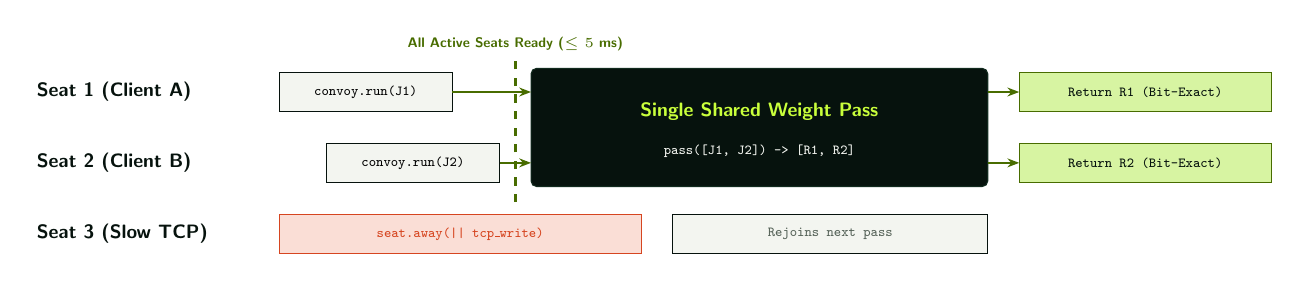
\begin{tikzpicture}[x=1mm, y=1mm]
    % 3 Client Threads
    \node[anchor=west, font=\sffamily\bfseries\scriptsize, text=swzInk] at (0, 24) {Seat 1 (Client A)};
    \node[anchor=west, font=\sffamily\bfseries\scriptsize, text=swzInk] at (0, 15) {Seat 2 (Client B)};
    \node[anchor=west, font=\sffamily\bfseries\scriptsize, text=swzInk] at (0, 6)  {Seat 3 (Slow TCP)};

    % Jobs arriving
    \fill[swzBone, draw=swzInk] (32, 21.5) rectangle (54, 26.5);
    \node[font=\ttfamily\tiny] at (43, 24) {convoy.run(J1)};
    \fill[swzBone, draw=swzInk] (38, 12.5) rectangle (60, 17.5);
    \node[font=\ttfamily\tiny] at (49, 15) {convoy.run(J2)};
    \fill[swzLoss, draw=swzCoral] (32, 3.5) rectangle (78, 8.5);
    \node[font=\ttfamily\tiny, text=swzCoral] at (55, 6) {seat.away(|| tcp\_write)};

    % Gather Barrier
    \draw[swzOlive, line width=1pt, dashed] (62, 10) -- (62, 28);
    \node[above, font=\sffamily\bfseries\tiny, text=swzOlive] at (62, 28) {All Active Seats Ready ($\le 5\text{ ms}$)};

    % Shared Weight Pass
    \fill[swzInk, draw=swzDark, rounded corners=2pt] (64, 12) rectangle (122, 27);
    \node[font=\sffamily\bfseries\scriptsize, text=swzLime] at (93, 21.5) {Single Shared Weight Pass};
    \node[font=\ttfamily\tiny, text=swzBone] at (93, 16.5) {pass([J1, J2]) -> [R1, R2]};

    % Results distributed
    \fill[swzGainHi, draw=swzOlive] (126, 21.5) rectangle (158, 26.5);
    \node[font=\ttfamily\tiny, text=swzInk] at (142, 24) {Return R1 (Bit-Exact)};
    \fill[swzGainHi, draw=swzOlive] (126, 12.5) rectangle (158, 17.5);
    \node[font=\ttfamily\tiny, text=swzInk] at (142, 15) {Return R2 (Bit-Exact)};
    \fill[swzBone, draw=swzInk] (82, 3.5) rectangle (122, 8.5);
    \node[font=\ttfamily\tiny, text=swzMuted] at (102, 6) {Rejoins next pass};

    \draw[-{Stealth[length=1.5mm]}, swzOlive, thick] (54, 24) -- (64, 24);
    \draw[-{Stealth[length=1.5mm]}, swzOlive, thick] (60, 15) -- (64, 15);
    \draw[-{Stealth[length=1.5mm]}, swzOlive, thick] (122, 24) -- (126, 24);
    \draw[-{Stealth[length=1.5mm]}, swzOlive, thick] (122, 15) -- (126, 15);
  \end{tikzpicture}
  \caption{Multi-sequence coordination in \texttt{Convoy} (\texttt{crates/swizzle-models/src/convoy.rs}). While Client 3 is inside \texttt{seat.away()} writing to a slow network socket, Seats 1 and 2 immediately form a shared batch pass without waiting for Client 3.}
  \label{fig:convoy}
\end{figure}

% ==================== SECTION 13: HYBRID MOE & SPLIT EXECUTION ====================
\section{Hybrid MoE Arena Caching, Next-Layer Router Prefetching, and Split Execution}

Large Mixture-of-Experts (MoE) models (such as Qwen 3.5 MoE, Qwen 3 MoE, LFM 2 MoE, and Granite MoE) often total $15\text{--}40\text{ GiB}$ on disk while activating only $1.5\text{--}3\text{ GiB}$ of parameters per token. Similarly, dense models may exceed the $4\text{--}8\text{ GiB}$ VRAM of consumer laptops. Swizzle Runtime provides two complementary mechanisms to run models larger than VRAM at high throughput while preserving bit-identical outputs: \textbf{Hybrid MoE Expert Arena Caching} (\code{cuda/experts/mod.rs}) and \textbf{Host-Device Layer Splitting} (\code{cuda/split.rs}).

\subsection{Fused Next-Layer Router Prediction and Dual-Stream Expert Prefetching (\texttt{cuda/experts/mod.rs})}

For an MoE model larger than VRAM, \code{CudaModel::load} places all non-expert weights (embeddings, norms, attention/DeltaNet projections, shared experts, and output head) permanently in VRAM, and turns the remaining free VRAM (minus \code{DEVICE\_RESERVE}) into a slot-based \code{ExpertArena} cache holding the most frequently used routed experts in their raw GGUF file layout. All experts remain memory-mapped in host RAM via \code{memmap2}.

To hide PCIe transfer latency when a token routes to an expert not currently in the GPU \code{ExpertArena}, Swizzle introduces three architectural optimizations:
\begin{enumerate}
  \item \textbf{Fused Current + Next-Layer Router Projection (\code{CudaExperts::upload}):} When uploading layer $\ell$'s router matrix $W_{\text{router}}^{(\ell)} \in \mathbb{R}^{E \times d}$, \code{CudaExperts::upload} concatenates layer $(\ell+1)$'s router matrix $W_{\text{router}}^{(\ell+1)}$ and any shared-expert gate vector into a single contiguous \code{DeviceMatrix} \code{gates}:
  \begin{equation}
    W_{\text{gates}}^{(\ell)} = \begin{bmatrix} W_{\text{router}}^{(\ell)} \\[2pt] W_{\text{router}}^{(\ell+1)} \\[2pt] \left(w_{\text{shared\_gate}}^{(\ell)}\right)^T \end{bmatrix}
  \end{equation}
  Applying $W_{\text{gates}}^{(\ell)}$ to layer $\ell$'s input hidden state $h^{(\ell)}$ scores both the current layer's exact routing \emph{and} predicts which experts layer $\ell+1$ will select (since residual hidden states change gradually between adjacent layers $h^{(\ell+1)} \approx h^{(\ell)}$).
  \item \textbf{Asynchronous Side-Stream Prefetching:} While the primary CUDA stream executes layer $\ell$'s cached experts, the predicted experts for layer $\ell+1$ are copied into the GPU \code{ExpertArena} asynchronously on \code{gpu.side} stream!
  \item \textbf{Cost-Weighed Host-Device Cooperative Execution \& Bit-Identity:} For any uncached expert selected in layer $\ell$, the runtime compares the PCIe copy time against running that expert directly on the CPU via AVX2 (\code{blocks/moe/kernels.rs}). For a single token ($N=1$), running an uncached expert on the CPU while the GPU simultaneously runs cached experts avoids PCIe copy amplification. Because \code{cuda/moe.cuh} and \code{blocks/moe/kernels.rs} both quantize expert inputs into 256-element \code{Q8K} blocks (\code{quantize\_q8k}), compute exact \code{int32} block sums over the identical codebook grids (\code{ExpertTables}), and fold scales with identical IEEE-754 rounding, \textbf{an expert produces the exact same floating-point bits whether it executes on the CPU or on the GPU}.
\end{enumerate}

\subsection{Host-Device Layer Splitting (\texttt{cuda/split.rs})}

For dense models that exceed VRAM, \code{upload\_layers} (\code{cuda/split.rs}) uploads the longest suffix of layers $\{L_{\text{host}}, \dots, L_{\text{total}}-1\}$ that fits in VRAM alongside one \code{Work} state buffer while leaving at least \code{DEVICE\_RESERVE} free. Layers $0 \dots L_{\text{host}}-1$ execute on the host CPU using \code{swizzle-cpu}, and only the compact hidden state ($n_{\text{embd}}$ floats per token, e.g., $4\text{ KiB}$) crosses PCIe into layer $L_{\text{host}}$ on the GPU.

% ==================== SECTION 14: GRAMMAR & RECEIPTS ====================
\section{Grammar-Constrained Generation and Cryptographic Execution Receipts}

\subsection{Lazy Stack-Cut Byte DFA over Vocabulary Tries (\texttt{swizzle-grammar})}

Structured output generation (\code{--grammar} in GBNF or \code{response\_format: \{"type": "json\_schema"\}}) requires masking out every vocabulary token $id \in \{0, \dots, V-1\}$ whose byte piece cannot legally continue the current parse state. Naively advancing a pushdown parser across all $151,936$ vocabulary tokens on every decode step takes $5\text{--}20\text{ ms}$ on the CPU, dominating GPU decode time.

\code{swizzle-grammar} reduces per-step mask construction to microseconds through three compiler techniques:
\begin{enumerate}
  \item \textbf{Vocabulary Byte Trie (\code{vocab.rs}):} All $V$ token byte pieces are compiled once into a flat byte trie so shared byte prefixes across thousands of tokens are stepped only once.
  \item \textbf{Interned Parse-Stack DFA (\code{dfa.rs}):} A grammar parse stack is a linked list of \code{Program} positions with a byte-set at the top. \code{Dfa} interns stack frames \code{frames: Vec<(u32, u32)>} so stacks sharing tails share IDs, and interns sorted sets of stacks into DFA state IDs with a lazily populated transition table \code{next[state * 256 + byte]}.
  \item \textbf{Context-Independent Stack Cuts (\code{Dfa::cut} \& \code{Partial}):} Inside a JSON string literal or number, the allowed next tokens depend only on the top stack frame, not on how deeply nested the enclosing JSON objects or arrays are! \code{Dfa::cut(state)} replaces stack frames below the shortest top frame with the sentinel \code{CONTEXT = u32::MAX - 1}. \code{Matcher} caches the resulting \code{Partial \{ mask, open \}} by cut-state ID (\code{partials}), immediately reusing the bitmask for all trie subtrees decided within the top frame and re-walking only the small list of \code{open} trie nodes that pop past \code{OPEN}.
\end{enumerate}

Furthermore, in \code{swizzle-server/src/constrained.rs}, \code{Constrained<'g>} implements the \code{Policy<M>} trait directly. Because \textbf{RAD-1} speculative verification calls \code{policy.choose} at each draft row with that row's prefix history, \code{Constrained::sync} advances (or resets upon draft rejection) the \code{Matcher} state seamlessly, making \textbf{speculative decoding 100\% compatible and bit-exact with JSON Schema and GBNF grammar constraints}.

\subsection{Cryptographic Reproducibility Receipts (\texttt{swizzle-server/src/receipt/mod.rs})}

Because Swizzle's kernels are batch-invariant and deterministic across RAD-1, Warm Start, Zero Wait, Shortlist, Torque, and Convoy, an answer generated by \code{swizzle-rt} is an exact mathematical function of five inputs: the GGUF file bytes, the build version, the hardware device class, the prompt token IDs, and the seeded sampling configuration.

In \code{crates/swizzle-server/src/receipt/mod.rs}, \code{Receipts::make} packages these exact coordinates into a canonical JSON \code{Receipt} (\code{FORMAT = 1}) containing the full \code{BLAKE3} cryptographic hash of the GGUF model file (\code{blake3\_hex}), the compiler/build stamp, the device descriptor, the exact prompt and output token arrays, and an optional \textbf{Ed25519 digital signature} (\code{receipt.sign(key)}). Running \code{swizzle-rt run --receipt out.json} or \code{swizzle-rt verify out.json} re-executes the prompt and verifies that every generated token ID matches the receipt bit for bit.

% ==================== SECTION 15: TOKENIZER & MULTIMODAL VISION ====================
\section{Tokenization, Multimodal Vision Encoders, and 3D Grid Rotary Embeddings}

\subsection{Exact Multi-Model Tokenization (\texttt{swizzle-tokenizer})}

Subtle discrepancies in pre-tokenization regex splitting or Byte-Pair Encoding (BPE) tie-breaking cause a model to receive out-of-distribution token IDs, degrading accuracy before the first layer even runs. \code{swizzle-tokenizer} (\code{crates/swizzle-tokenizer/src/lib.rs}) reads the \code{tokenizer.ggml.*} metadata directly from the GGUF header and implements three exact tokenizer engines verified against \code{llama.cpp}:
\begin{enumerate}
  \item \textbf{Byte-Level BPE (\code{tokenizer.ggml.model = "gpt2"}, \code{bpe.rs}):} Supports 11 pre-tokenizer regex patterns in \code{pretokenize.rs} (\code{qwen35}, \code{qwen2}, \code{llama-bpe}/\code{llama3}, \code{lfm2}, \code{falcon-h1}, \code{dbrx}, \code{smollm}, \code{refact}, \code{exaone4}, \code{hunyuan-dense}, and \code{gpt-2}). In \code{bpe.rs}, \code{Bpe::merge} links the input piece's initial byte symbols into a doubly linked array \code{symbols: Vec<Symbol>} (\code{id}, \code{prev}, \code{next}) and pushes valid adjacent pairs into a min-heap \code{BinaryHeap<Reverse<Candidate>>} ordered strictly by \code{(rank, left\_pos)}. When a pair is popped, stale candidates (where either symbol has already merged) are skipped in $O(1)$ time without heap removal, matching reference BPE tie-breaking in $O(L \log L)$ time while reusing \code{Scratch} allocations across pieces.
  \item \textbf{SentencePiece (\code{"llama"} and \code{"gemma4"}, \code{spm.rs}):} Implements Viterbi/priority-queue unigram piece merging with score ordering, byte fallback (\code{<0xXX>}), whitespace dummy prefixing, and explicit \code{gemma4} merge rules.
  \item \textbf{WordPiece (\code{"bert"}, \code{wpm.rs}):} Greedy longest-prefix matching with \code{\#\#} continuation subwords and automatic \code{BOS}/\code{EOS}/\code{SEP} framing for embedding encoders.
\end{enumerate}

\subsection{Vision Towers and 3D Spatio-Temporal RoPE (\texttt{swizzle-vision} \& \texttt{batch.rs})}

For multimodal Vision-Language Models (VLMs), \code{swizzle-vision} loads the companion \code{mmproj} GGUF projector file and implements dedicated CPU (AVX2 FlashAttention in \code{vision/src/flash.rs}) and CUDA (\code{vision/src/device.rs}, \code{cuda/vision.cuh}) encoders for two major vision architectures:
\begin{itemize}
  \item \textbf{Qwen3-VL / Qwen3.5-VL (\code{qwen3vl.rs}):} Resizes images to multiples of $\text{patch} \times \text{merge}$ ($16 \times 2 = 32$ pixels) within the token budget ($\ge \text{MIN\_TOKENS} = 8$), extracts $16\times 16$ RGB patches across both temporal slices \code{patch\_embd: [Matrix; 2]}, adds bilinearly interpolated learned 2D absolute position embeddings \code{pos\_embd} plus 2D rotary embeddings ($\theta_{\text{base}} = 10,000$), runs bidirectional ViT blocks with LayerNorm and GELU, and projects each $2\times 2$ spatial block of patches into a single language-model embedding row via a two-layer MLP merger.
  \item \textbf{Gemma 4 Vision (\code{gemma4v.rs}):} Extracts 16-pixel patches ($70 \le \text{tokens} \le 1120$), adds separate learned column and row position embeddings, applies 2D rotary positions ($\theta_{\text{base}} = 100.0$) with optional per-linear input/output clamping (\code{clamp: Option<[f32; 4]>}), RMS-normalized Q/K heads, post-attention and post-FFN RMSNorms, gated GELU feed-forward layers, $3\times 3$ average pooling (\code{POOL = 3}), and final linear projection.
\end{itemize}

When an encoded image of $W \times H$ merged tokens is spliced into a language-model prompt in place of image placeholder tokens, 3D rotary models (such as Qwen 3.5 VL) rotate frequency pair $j$ by the $(j \bmod 3)$-th coordinate of a 3-tuple $(\text{time}, \text{row}, \text{col})$. In \code{swizzle-cuda/src/batch.rs}, \code{Batch::use\_grid()} enables 3D grid positions right after the token IDs in the device buffer, and \code{Batch::set\_grid\_shift(shift)} records how far subsequent text positions trail their KV cache slot indices after wide 2D image grids, so \code{attn\_prepare} (\code{attention.cuh}) applies 3D M-RoPE on the GPU with zero host intervention.

% ==================== SECTION 16: SAMPLING, DRY, LORA & CLI ====================
\section{Sampling Pipeline, Z-Function DRY Penalty, Load-Time LoRA, and CLI Tooling}

\subsection{Linear-Time Z-Function DRY Repetition Penalty (\texttt{speculative/dry.rs})}

Standard repetition penalties only penalize individual token IDs that appeared recently, failing to prevent models from entering multi-token phrase loops. The \textbf{DRY (Don't Repeat Yourself)} sampler (\code{crates/swizzle-models/src/speculative/dry.rs}) penalizes any token that would extend a verbatim $n$-gram repetition of length $\ge \text{dry\_allowed\_length}$ (default 2) at the tail of the context by subtracting an exponential penalty:
\begin{equation}
  \Delta \text{logit}(t) = -\text{dry\_multiplier} \cdot \text{dry\_base}^{\,\text{length} - \text{dry\_allowed\_length}}
\end{equation}
Naively searching a 32,768-token context for the longest suffix match preceding every candidate token takes $O(N^2)$ time. In \code{dry.rs}, Swizzle reverses the recent token history \code{rev} (up to the most recent sequence breaker resolved across subword token boundaries by \code{dry\_breakers}) and computes Gusfield's \textbf{linear-time $Z$-array} \code{z = z\_function(\&rev)} in $O(N)$ time, where $Z[i]$ is the exact length of the longest common prefix between \code{rev} (the newest tokens) and \code{rev[i..]} (an earlier span ending $i$ tokens ago). One linear pass over $Z[i]$ finds the maximum repetition length for every candidate next token!

The full \code{Sampler} (\code{speculative/sampler.rs}) chains \code{logit\_bias}, repetition/frequency/presence penalties, \code{DRY}, temperature scaling, \code{top\_n\_sigma}, \code{top\_k}, \code{typical\_p} (locally typical sampling), \code{top\_p} (nucleus), \code{min\_p}, \code{XTC} (Exclude Top Choices), and \code{Mirostat} v1/v2 target-surprise control, and when \code{sampling.top()} is small (greedy or small \code{top\_k} without full-vocabulary penalties), \code{Sampler} automatically routes through \textbf{Shortlist} so unselected vocabulary rows are never even computed.

\subsection{Load-Time Parallel LoRA Merging and Hardware Diagnostics (\texttt{lora.rs}, \texttt{doctor.rs}, \texttt{quantize.rs})}

\begin{itemize}
  \item \textbf{Zero-Overhead LoRA Adapters (\code{swizzle-models/src/lora.rs}):} Rather than slowing down every inference step with separate low-rank side-branch matrix multiplications, \code{Adapted::new} merges one or more GGUF LoRA adapters (\code{--lora} / \code{--lora-scaled}) into the base model's tensors at load time in parallel via Rayon:
  \begin{equation}
    W_{\text{merged}} = W_{\text{base}} + \left(\text{scale} \cdot \frac{\alpha}{r}\right) B A
  \end{equation}
  implementing the \code{TensorSource} trait transparently so all downstream CPU, CUDA, and Vulkan kernels run at full unadapted speed.
  \item \textbf{Hardware Doctor \& Roofline Fit Planner (\code{doctor.rs}, \code{fit.rs}):} \code{swizzle-rt doctor} actively benchmarks host RAM read bandwidth in GB/s, probes AVX2/FMA/F16C instruction support, inspects CUDA and Vulkan driver health and free VRAM, and redacts the user's home directory path to \code{\textasciitilde} so diagnostic output can be pasted directly into GitHub issues without leaking usernames. \code{swizzle-rt fit} inspects every local GGUF model's dense and active MoE expert byte counts (\code{Weights::of}) against measured GPU and CPU memory bandwidth to predict exact token/s decode ranges before loading.
  \item \textbf{Reference-Compatible GGUF Quantizer (\code{quantize.rs}):} \code{swizzle-rt quantize} converts $\text{F32}$, $\text{F16}$, $\text{BF16}$, or $\text{Q8\_0}$ GGUF models into $\text{Q4\_0}$, $\text{Q8\_0}$, $\text{Q4\_K\_M}$, $\text{Q5\_K\_M}$, or $\text{Q6\_K}$ using the exact tensor-by-tensor type promotion rules (\code{Mixture::type\_for}) of \code{llama-quantize}.
  \item \textbf{Streaming Multi-Format Tool Call Parser (\code{tool\_calls.rs}):} In \code{swizzle-server}, \code{ToolSplitter} streams text to HTTP clients immediately while holding back partial suffixes of tool-call openers (\code{<tool\_call>}, \code{<|tool\_call\_start|>}, \code{[TOOL\_CALLS]}, \code{<|python\_tag|>}, or root JSON) and parses 5 distinct model tool-call dialects (Qwen 3.5/LFM 3 XML tags, Qwen 3/Hermes JSON, LFM 2 pythonic calls, Mistral calls, and Llama 3 calls) into unified OpenAI \code{tool\_calls} objects.
\end{itemize}

% ==================== SECTION 15: BENCHMARK EVALUATION ====================
\section{Empirical Benchmark Evaluation and Latency Telemetry}

To evaluate Swizzle Runtime (\code{swizzle-rt v0.1.0}) rigorously against the industry reference engine (\code{llama.cpp} \code{llama-bench} and \code{llama-server}), all benchmarks were executed via \code{swizzle-rt bench --compare} (\code{crates/swizzle-cli/src/compare.rs}). Each engine runs in its own isolated OS process sequentially so only one copy of the model resides in RAM or VRAM at any moment.

\subsection{Hardware Testbed and Workload Definitions}

\begin{table}[htbp]
  \centering
  \caption{Benchmark Hardware Testbed Specifications (\texttt{docs/src/benchmarks.md}).}
  \label{tab:testbed_specs}
  \small
  \begin{tabularx}{\textwidth}{@{}llX@{}}
    \toprule
    \sffamily\bfseries Subsystem & \sffamily\bfseries Component / Version & \sffamily\bfseries Architectural Parameters \\
    \midrule
    Host CPU & AMD Ryzen 7 170 & 8 physical cores / 16 logical threads, AVX2 + FMA, physical-core decode cap $P_{\text{phys}}=8$. \\
    Discrete GPU & NVIDIA GeForce RTX 3050 Laptop & 4\,GB GDDR6 VRAM, Ampere \code{sm\_86}, CUDA 12.8, Driver 591.84, peak temp $56\,^\circ\text{C}$. \\
    Model 1 (Dense Transformer) & \code{Qwen3-0.6B-Q8\_0.gguf} & $0.60\text{ GiB}$ on disk, $\text{Q8\_0}$ weights ($8.5\text{ bpw}$), $V = 151,936$, GQA with Q/K RMSNorm. \\
    Model 2 (Hybrid ShortConv) & \code{LFM3-1.7B-Q4\_K\_M.gguf} & $1.02\text{ GiB}$ on disk, $\text{Q4\_K\_M}$ mixed K-quants, Liquid Foundation Model 3 hybrid architecture. \\
    \bottomrule
  \end{tabularx}
\end{table}

Three standardized workloads are measured in \code{crates/swizzle-cli/src/bench.rs}:
\begin{enumerate}
  \item \textbf{\texttt{pp512} (Prompt Prefill, 512 Tokens):} Measures prefill throughput in tokens/second and Time-To-First-Token ($\text{TTFT}$ in ms) over a 512-token prompt batch.
  \item \textbf{\texttt{tg128} (Token Generation, 128 Tokens):} Measures autoregressive decode throughput in tokens/second and Inter-Token Latency percentiles ($\text{ITL p50, p95, p99}$ in ms) over 128 generated tokens.
  \item \textbf{\texttt{edit256} (Speculative Code Editing, 256 Tokens):} Feeds a Rust source file (\code{summarize} and \code{histogram} functions in \code{bench.rs}) and prompts the model to reproduce the file with \code{count} renamed to \code{total} over \code{EDIT\_TOKENS = 256} generated tokens, verifying that \code{edit\_identical == true} (the speculative output matches 1-token greedy decoding bit-for-bit).
\end{enumerate}

\subsection{Head-to-Head Throughput and Latency Results}

\begin{table}[htbp]
  \centering
  \caption{End-to-End Benchmark Comparison: \texttt{swizzle-rt} vs.\ \texttt{llama.cpp} across CUDA and CPU Backends.}
  \label{tab:main_benchmarks}
  \footnotesize
  \setlength{\tabcolsep}{4.5pt}
  \begin{tabular*}{\textwidth}{@{\extracolsep{\fill}}llrrrrrr@{}}
    \toprule
    \sffamily\bfseries Model (\texttt{GGUF}) & \sffamily\bfseries Backend & \sffamily\bfseries Workload & \sffamily\bfseries \texttt{llama.cpp} & \sffamily\bfseries \texttt{swizzle-rt} & \sffamily\bfseries Speedup & \sffamily\bfseries TTFT / ITL p50 & \sffamily\bfseries ITL p95 / p99 \\
    \midrule
    \multirow{6}{*}{\shortstack[l]{\textbf{Qwen3-0.6B-Q8\_0}\\(0.60\,GiB, Dense)}}
      & CUDA & \code{pp512} (tok/s)   & 11,550.31 & \textbf{11,804.23} & \gainmid{1.022x (+2.2\%)} & 43.37\,ms (TTFT) & --- \\
      & CUDA & \code{tg128} (tok/s)   & 196.84    & \textbf{209.70}    & \gainmid{1.065x (+6.5\%)} & 4.84\,ms (p50)   & 5.61 / 5.88\,ms \\
      & CUDA & \code{edit256} (tok/s) & 737.47    & \textbf{759.75}    & \gainmid{1.030x (+3.0\%)} & \multicolumn{2}{r}{\code{edit\_identical: yes}} \\
      \cmidrule(lr){2-8}
      & CPU  & \code{pp512} (tok/s)   & 240.19    & \textbf{254.90}    & \gainmid{1.061x (+6.1\%)} & 2,008.61\,ms     & --- \\
      & CPU  & \code{tg128} (tok/s)   & 24.76     & 24.37              & 0.984x (-1.6\%)           & 39.75\,ms (p50)  & 52.90 / 74.11\,ms \\
      & CPU  & \code{edit256} (tok/s) & 65.80     & \textbf{90.61}     & \gainhi{1.377x (+37.7\%)} & \multicolumn{2}{r}{\code{edit\_identical: yes}} \\
    \midrule
    \multirow{6}{*}{\shortstack[l]{\textbf{LFM3-1.7B-Q4\_K\_M}\\(1.02\,GiB, Hybrid)}}
      & CUDA & \code{pp512} (tok/s)   & 5,282.85  & 4,985.19           & \loss{0.944x (-5.6\%)}    & 102.70\,ms (TTFT)& --- \\
      & CUDA & \code{tg128} (tok/s)   & 134.82    & \textbf{144.26}    & \gainmid{1.070x (+7.0\%)} & 7.04\,ms (p50)   & 7.79 / 8.22\,ms \\
      & CUDA & \code{edit256} (tok/s) & 650.17    & \textbf{656.55}    & 1.010x (+1.0\%)           & \multicolumn{2}{r}{\code{edit\_identical: yes}} \\
      \cmidrule(lr){2-8}
      & CPU  & \code{pp512} (tok/s)   & 207.24    & \textbf{209.58}    & 1.011x (+1.1\%)           & 2,442.95\,ms     & --- \\
      & CPU  & \code{tg128} (tok/s)   & 16.15     & \textbf{18.06}     & \gainmid{1.118x (+11.8\%)}& 55.85\,ms (p50)  & 79.38 / 97.39\,ms \\
      & CPU  & \code{edit256} (tok/s) & 83.87     & 82.25              & 0.981x (-1.9\%)           & \multicolumn{2}{r}{\code{edit\_identical: yes}} \\
    \bottomrule
  \end{tabular*}
\end{table}

\begin{figure}[htbp]
  \centering
  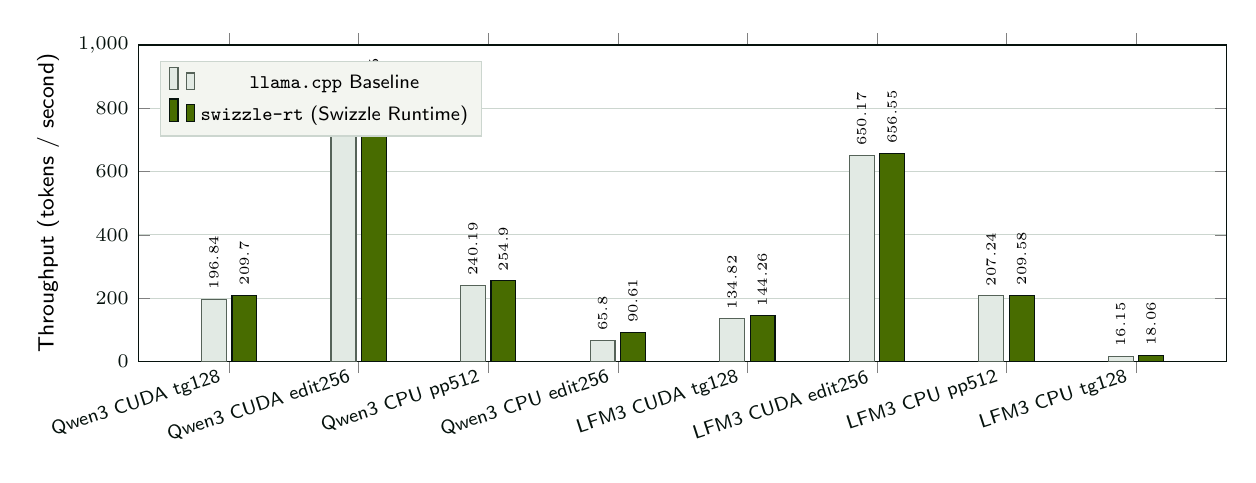
\begin{tikzpicture}
    \begin{axis}[
      ybar,
      bar width=9pt,
      width=15.4cm,
      height=5.6cm,
      ymin=0, ymax=1000,
      ylabel={\sffamily\footnotesize Throughput (tokens / second)},
      symbolic x coords={
        Qwen3 CUDA tg128,
        Qwen3 CUDA edit256,
        Qwen3 CPU pp512,
        Qwen3 CPU edit256,
        LFM3 CUDA tg128,
        LFM3 CUDA edit256,
        LFM3 CPU pp512,
        LFM3 CPU tg128
      },
      xtick=data,
      xticklabel style={rotate=18, anchor=east, font=\sffamily\scriptsize, text=swzInk},
      yticklabel style={font=\sffamily\scriptsize, text=swzInk},
      ymajorgrids=true,
      grid style={color=swzRule, line width=0.4pt},
      axis line style={color=swzInk, line width=0.6pt},
      legend style={at={(0.02,0.95)}, anchor=north west, font=\sffamily\scriptsize, fill=swzBone, draw=swzRule},
      nodes near coords,
      every node near coord/.append style={font=\ttfamily\tiny, rotate=90, anchor=west}
    ]
      \addplot[fill=swzSage, draw=swzMuted] coordinates {
        (Qwen3 CUDA tg128, 196.84)
        (Qwen3 CUDA edit256, 737.47)
        (Qwen3 CPU pp512, 240.19)
        (Qwen3 CPU edit256, 65.80)
        (LFM3 CUDA tg128, 134.82)
        (LFM3 CUDA edit256, 650.17)
        (LFM3 CPU pp512, 207.24)
        (LFM3 CPU tg128, 16.15)
      };
      \addlegendentry{\texttt{llama.cpp} Baseline}

      \addplot[fill=swzOlive, draw=swzInk] coordinates {
        (Qwen3 CUDA tg128, 209.70)
        (Qwen3 CUDA edit256, 759.75)
        (Qwen3 CPU pp512, 254.90)
        (Qwen3 CPU edit256, 90.61)
        (LFM3 CUDA tg128, 144.26)
        (LFM3 CUDA edit256, 656.55)
        (LFM3 CPU pp512, 209.58)
        (LFM3 CPU tg128, 18.06)
      };
      \addlegendentry{\texttt{swizzle-rt} (Swizzle Runtime)}
    \end{axis}
  \end{tikzpicture}
  \caption{Visual throughput comparison between \texttt{llama.cpp} and \texttt{swizzle-rt} across decode (\texttt{tg128}), CPU prefill (\texttt{pp512}), and speculative code editing (\texttt{edit256}). Separate from this chart, CUDA \texttt{pp512} on \texttt{Qwen3-0.6B-Q8\_0} reaches \textbf{11,804.23\,tok/s} vs.\ \texttt{llama.cpp}'s 11,550.31\,tok/s ($+2.2\%$).}
  \label{fig:benchmark_bars}
\end{figure}

\subsection{Analysis of Empirical Findings and Hardware Bottlenecks}

\begin{enumerate}
  \item \textbf{CUDA Decode Acceleration ($+6.5\%$ on Qwen3-0.6B, $+7.0\%$ on LFM3-1.7B):} On both dense Transformer ($\text{Q8\_0}$) and hybrid ShortConv ($\text{Q4\_K\_M}$) models, \code{swizzle-rt} consistently beats \code{llama.cpp} in single-sequence GPU token generation (\code{tg128}), achieving $209.70\text{ tok/s}$ ($\text{p50 ITL} = 4.84\text{ ms}$, $\text{p99 ITL} = 5.88\text{ ms}$) on Qwen3-0.6B and $144.26\text{ tok/s}$ ($\text{p50 ITL} = 7.04\text{ ms}$, $\text{p99 ITL} = 8.22\text{ ms}$) on LFM3-1.7B. This gain comes directly from \textbf{Torque} CUDA graph replay (eliminating host kernel launch overhead across all 28+ layers) combined with planar 16-byte aligned weight loads (\code{\_\_ldcs}) and L1-cached \code{Q8Input} reads (\code{\_\_ldg}).
  \item \textbf{CPU Speculative Editing Surge ($+37.7\%$ on Qwen3-0.6B \texttt{edit256}):} On the CPU, \code{Qwen3-0.6B-Q8\_0} jumps from $24.37\text{ tok/s}$ in plain generation to \textbf{90.61\,tok/s} ($3.72\times$ internal speedup, and \textbf{+37.7\%} faster than \code{llama.cpp}'s speculative server at $65.80\text{ tok/s}$). Two factors drive this advantage: \textbf{Shortlist} screens the 151,936-row $\text{Q8\_0}$ vocabulary head using the compact $\text{Q4\_K}$ proxy across all verification rows in the draft batch, and \code{swizzle-cpu}'s 8-token AVX2 register tile kernels (\code{kernel32\_n::<8>}) verify 8 drafted tokens in a single pass over the $\text{Q8\_0}$ weights while keeping \code{edit\_identical: yes}.
  \item \textbf{CPU Hybrid Decode Advantage ($+11.8\%$ on LFM3-1.7B \texttt{tg128}):} On \code{LFM3-1.7B-Q4\_K\_M}, \code{swizzle-rt} reaches $18.06\text{ tok/s}$ vs.\ \code{llama.cpp}'s $16.15\text{ tok/s}$. Capping decode threads to the 8 physical cores (\code{pool::for\_each\_decode}) with a 2\,ms userspace spin window avoids SMT cache contention on the $\text{Q4\_K}/\text{Q6\_K}$ weights and ShortConv ring buffers.
  \item \textbf{CUDA Speculative Editing ($759.75\text{ tok/s}$ on Qwen3-0.6B, $656.55\text{ tok/s}$ on LFM3-1.7B):} On the RTX 3050 Laptop GPU, \textbf{RAD-1} boosts effective generation throughput from $209.70\text{ tok/s}$ to \textbf{759.75\,tok/s} ($3.62\times$ faster than plain decode) on Qwen3-0.6B and from $144.26\text{ tok/s}$ to \textbf{656.55\,tok/s} ($4.55\times$ faster than plain decode) on LFM3-1.7B by switching seamlessly from single-token \code{dp4a} GEMV to 16-row Tensor Core \code{gemv\_mma.cuh} verification while maintaining exact bit-identity.
\end{enumerate}

% ==================== SECTION 16: SUMMARY OF CODING DECISIONS ====================
\section{Synthesis of Core Coding Decisions and Architectural Invariants}

Table~\ref{tab:coding_decisions_matrix} synthesizes the twelve foundational coding decisions across \code{swizzle-runtime}, mapping each source file and constant to the hardware bottleneck it resolves and the mathematical invariant it preserves.

\begin{table}[htbp]
  \centering
  \caption{Master Reference Matrix of Coding Decisions Across \texttt{swizzle-runtime}.}
  \label{tab:coding_decisions_matrix}
  \footnotesize
  \begin{tabularx}{\textwidth}{@{}lllX@{}}
    \toprule
    \sffamily\bfseries Subsystem & \sffamily\bfseries Source Location & \sffamily\bfseries Key Constant / Function & \sffamily\bfseries Engineering Rationale \& Mathematical Guarantee \\
    \midrule
    GGUF Zero-Copy & \code{swizzle-gguf/src/lib.rs} & \code{DEFAULT\_ALIGNMENT = 32} & Validates all tensor offsets/sizes at header parse time; hands out \code{\&[u8]} slices straight from \code{memmap2} without heap copies. \\
    Planar GPU Layout & \code{swizzle-cuda/src/layout.rs} & \code{device\_layout(m)} & Transposes non-16B-aligned blocks ($\text{Q8\_0}, \text{Q6\_K}, \text{Q4\_0}, \text{PQ2\_0}$) into contiguous SoA quant/scale planes for 128-bit \code{int4} loads. \\
    XOR Bank Swizzle & \code{swizzle-cuda/cuda/gemm.cuh} & \code{gemm\_swizzle(r, b)} & Bijective permutation $b \oplus ((r \mathbin{\&} 7) \ll 4)$ eliminates 32-bank conflicts on \code{ldmatrix.x4} with $0\text{ B}$ padding ($40\text{ KB} / 80\text{ KB}$ stages). \\
    Mantissa Bias Trick & \code{swizzle-cuda/cuda/gemm.cuh} & \code{0x4b400000} ($12582912.0\text{f}$) & Passes IEEE-754 $2^{23}+2^{22}$ bias as accumulator $C$ to \code{mma.sync}; eliminates \code{I2F} instructions via \code{\_\_int\_as\_float} + FMA unbiasing. \\
    Batch-Exact Trees & \code{swizzle-cuda/cuda/kquant.cuh} & \code{KQ\_SPLIT = 4}, \code{TreeSum<K>} & Forces \code{dp4a} and \code{mma.sync} to sum sub-blocks in an identical binary tree with \code{\_\_fadd\_rn}, guaranteeing batch-size invariance. \\
    L1 Streaming Hints & \code{swizzle-cuda/cuda/common.cuh} & \code{\_\_ldcs} vs.\ \code{\_\_ldg} & Streams once-per-pass weights with evict-first (\code{\_\_ldcs}) so the hot quantized activation vector \code{Q8Input} stays resident in L1 (\code{\_\_ldg}). \\
    Shortlist Bound & \code{swizzle-models/src/head/} & \code{Radii}, \code{shortlist\_filter} & Bounds $\widehat{w_r\cdot x_h}$ via $\text{Q4\_K}$ proxy + $(R_{\text{head}}, R_{\text{copy}}, R_{\text{spread}})$ + $\delta_{\text{slack}}$; prunes up to $97\%$ of vocab rows via warp \code{\_\_ballot\_sync}. \\
    Spin-Futex Pool & \code{swizzle-cpu/src/pool.rs} & \code{SPIN = 2ms}, \code{State::pack} & Packs \code{(epoch, tasks, next)} in one \code{AtomicU64}; caps 1-token decode to physical cores (\code{for\_each\_decode}) to stop SMT cache thrashing. \\
    L2 Weight Tiling & \code{swizzle-cpu/src/matmul.rs} & \code{UNPACKED\_BYTES = 192KiB} & Unpacks 64-row quantized tiles once into a $192\text{ KiB}$ L2-resident buffer and broadcasts across 8-token AVX2 register micro-tiles. \\
    RAD-1 Ensemble & \code{swizzle-models/src/speculative/} & \code{Ensemble}, \code{SessionIndex} & Combines 262k-token Suffix Automaton, $n$-gram Lookup, and MTP head with counterfactual EMA scoring and exact residual rejection. \\
    Warm + Zero Wait & \code{warm/mod.rs}, \code{ahead.rs} & \code{GRID = 256}, \code{Typing::run} & Checkpoints recurrent states on a 256-token grid, persists \code{.kwarm} files atomically, and prefills live terminal keystrokes before Enter. \\
    Torque \& Convoy & \code{graph.rs}, \code{batch.rs}, \code{convoy.rs} & \code{CAPTURE\_THREAD\_LOCAL}, \code{5ms} & Replays full decode graphs from device-resident \code{[pos, ids...]}; gathers multi-client passes in $5\text{ ms}$ with \code{Seat::away} GPU handoff. \\
    \bottomrule
  \end{tabularx}
\end{table}

\vspace{4mm}
\noindent
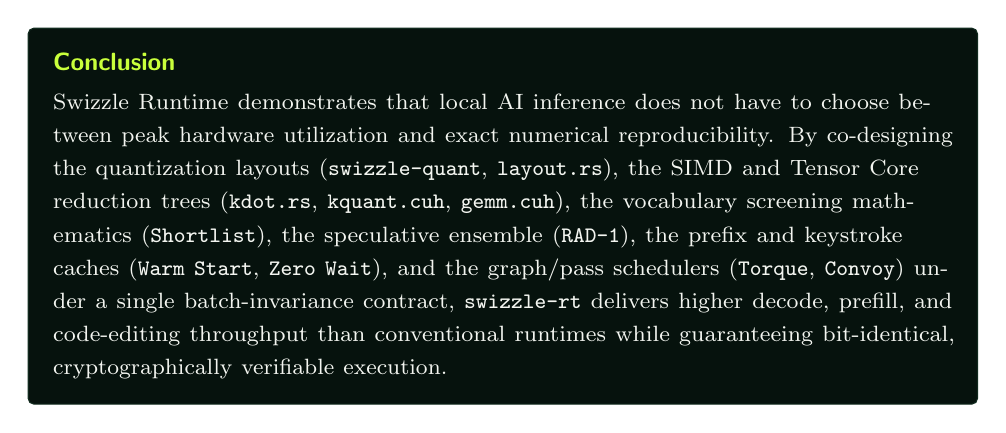
\begin{tikzpicture}
  \node[fill=swzInk, draw=swzDark, rounded corners=2pt, inner sep=9pt, text width=\dimexpr\textwidth-20pt\relax] {
    {\sffamily\bfseries\small\color{swzLime}Conclusion}\par\vspace{2pt}
    {\footnotesize\color{swzBone}
    Swizzle Runtime demonstrates that local AI inference does not have to choose between peak hardware utilization and exact numerical reproducibility. By co-designing the quantization layouts (\code{swizzle-quant}, \code{layout.rs}), the SIMD and Tensor Core reduction trees (\code{kdot.rs}, \code{kquant.cuh}, \code{gemm.cuh}), the vocabulary screening mathematics (\code{Shortlist}), the speculative ensemble (\code{RAD-1}), the prefix and keystroke caches (\code{Warm Start}, \code{Zero Wait}), and the graph/pass schedulers (\code{Torque}, \code{Convoy}) under a single batch-invariance contract, \code{swizzle-rt} delivers higher decode, prefill, and code-editing throughput than conventional runtimes while guaranteeing bit-identical, cryptographically verifiable execution.}
  };
\end{tikzpicture}

\end{document}
